\documentclass[12pt,twoside,openright,final]{report}
\usepackage{StyleCent}

\usepackage[utf8]{inputenc}
\usepackage[slovene]{babel}
\usepackage[intlimits]{amsmath}
\usepackage{hyperref}
\usepackage[nottoc,numbib]{tocbibind}
\usepackage{gensymb}
\usepackage[left=3cm,right=3cm,top=3cm,bottom=3cm]{geometry}
\usepackage{microtype}

\usepackage{graphicx}
\usepackage{subfigure}
\usepackage{comment}
\usepackage[smaller]{acronym}
\usepackage[percent]{overpic}
\usepackage{titlesec}
\usepackage{setspace}
\usepackage{dashrule}

\usepackage{tikz}
\usetikzlibrary{calc}

\tikzset{egrid/.style={draw,help lines}}
\tikzset{mgrid/.style={draw,help lines,dashed}}
\tikzset{epoint/.style={draw,circle,red,inner sep=2pt,fill}}
\tikzset{mpoint/.style={draw,circle,blue,inner sep=2pt,fill}}

\newcommand{\todo}[1]{(\textbf{\textsmaller{TODO}: #1})}
\newcommand{\odvod}[2]{\frac{\partial #1}{\partial #2}}
\renewcommand{\vec}{\mathbf}
\newcommand{\eps}{\varepsilon}
\newcommand{\E}{\vec E}
\newcommand{\B}{\vec B}
\newcommand{\angl}[1]{(\textit{angl. #1})}

\acrodef{FDTD}{Finite-difference time-domain}
\acrodef{ABC}{Absorbing boundary condition}
\acrodef{PML}{Perfectly-matched layer}

\renewcommand{\acf}[1]{\aclu{#1} -- \acs{#1}}
\newcommand{\dd}{\ensuremath{\;\mathrm{d}}}

\newcommand{\ticssize}{\fontsize{9}{10}\selectfont}
\newcommand{\qodv}[2]{\ensuremath{\frac{\partial Q_{#1}}{\partial x_{#2}}}}
\newcommand{\nodv}[2]{\ensuremath{\frac{\partial n_{#1}}{\partial x_{#2}}}}

\graphicspath{{./Slike/}}

\newcommand{\Authands}{ in }

\newcommand{\stalno}[2]{
  \begin{overpic}[width=.4\textwidth]{lic_#1_1}\put(2,90){\color{white} \large \bf (a)}\end{overpic} \hspace{1mm}
  \begin{overpic}[width=.4\textwidth]{lic_#1_37}\put(2,90){\color{white} \large \bf (b)}\end{overpic} \\[2.5mm]
  \begin{overpic}[width=.4\textwidth]{lic_#1_50}\put(2,90){\color{white} \large \bf (c)}\end{overpic} \hspace{-.5mm}
  \begin{overpic}[width=.4\textwidth,trim=-1cm -1cm -1cm -1cm]{g_defect_#2}\put(2,90){\large \bf (d)}\end{overpic}
}

\newcommand{\sunek}[1]{
  \begin{overpic}[width=.4\textwidth]{licp_#1_74}\put(2,90){\color{white} \large \bf (a)}\end{overpic} \hspace{1mm}
  \begin{overpic}[width=.4\textwidth]{licp_#1_82}\put(2,90){\color{white} \large \bf (b)}\end{overpic}
}

%opening
\title{Magistrsko delo}
\author{Miha \v Can\v cula}

\begin{document}

\thispagestyle{empty}
\begin{center}
{\Large\sc Univerza v Ljubljani \\
\medskip
Fakulteta za matematiko in fiziko\\
\medskip
Oddelek za fiziko}\\

\vfill

\bigskip\bigskip\bigskip\bigskip\bigskip\bigskip\bigskip\bigskip
\bigskip\bigskip\bigskip

{\Large Miha "Can"cula}\\

\bigskip\bigskip\bigskip

{\LARGE\sc {\bf Modeliranje "sirjenja svetlobe vzdol"z}}

\bigskip

{\LARGE\sc {\bf ograjenih teko"cekristalnih defektnih linij}}

\vskip 8mm \hrule height0.5mm \vskip 12mm

%\bigskip\bigskip

{\Large Magistrsko delo}\\

\bigskip\bigskip\bigskip\bigskip\bigskip\bigskip\bigskip\bigskip\bigskip\bigskip\bigskip\bigskip\bigskip\bigskip\bigskip

{\Large MENTOR: prof. dr. Slobodan "Zumer}\\ \smallskip\smallskip\smallskip

{\Large SOMENTOR: doc. dr. Miha Ravnik}

\bigskip\bigskip

\vfill
{\Large Ljubljana, 2013}
\end{center}

\newpage

\newpage

\thispagestyle{empty}

\centerline{}

\vfill

\centerline{\bf Izjava o avtorstvu in objavi elektronske oblike zaklju"cnega dela}
\bigskip\bigskip
\noindent


Podpisani Miha "Can"cula, rojen 10.~4.~1989 v Postojni, izjavljam:

\begin{itemize}
 \item da sem magistrsko delo z naslovom \emph{Modeliranje "sirjenja svetlobe vzdol"z ograjenih teko"cekristalnih defektnih linij} izdelal samostojno pod mentorstvom prof. dr. Slobodana "Zumra in somentorstvom doc. dr. Miha Ravnika in
 \item da Fakulteti za matematiko in fiziko Univerze v Ljubljani dovoljujem objavo \\ elektronske oblike svojega dela na spletnih straneh. 
\end{itemize}
 
\bigskip
\bigskip

\noindent
Ljubljana, 4.~9.~2013 \hfill Miha "Can"cula

\vfill

\newpage

\normalsize
\thispagestyle{empty}
\centerline{}
\vfill

\vfill

\vfill

\vfill


\par{\narrower\narrower\narrower\parindent 0pt

Iskreno se zahvaljujem mentorju, prof.~dr.~Slobodanu "Zumru, in somentorju, doc.~dr.~Mihu Ravniku, za strokovno vodstvo in pomo"c pri uvajanju v raziskovalno delo.

\quad

Zahvala gre tudi Davidu Se"cu, dr.~Tinetu Porenti in dr.~Simonu "Coparju, ki so mi ves "cas pisanja sedeli ob strani s koristnimi nasveti in pripombami. 

\par}

\vfill




\newpage

\normalsize
\thispagestyle{plain}

\vfill
\centerline{\bf Povzetek}
\bigskip
\noindent

Magistrsko delo obravnava "sirjenje svetlobe po teko"cekristalnih vlaknih z razli"cnimi direktorskimi profili. 
Opisan je razvoj numeri"cne metode za modeliranje propagacije elektromagnetnih polj skozi opti"cno anizotropna sredstva, kjer se dielektri"cni tenzor poljubno spreminja po prostoru. 
Postopek re"sevanja temelji na metodi kon"cnih diferenc v "casovni domeni. 
Teko"ci kristal je modeliran kot enoosno dvolomna snov s krajevno odvisno opti"cno osjo.
Izra"cunamo prepustnost plasti teko"cega kristala med prekri"zanima polarizatorjema, fotonski prepovedani pas v periodi"cni strukturi in lastne na"cine "sirjenja svetlobe v opti"cno anizotropnem vlaknu. 
Prepoznamo lastne na"cine valovanja v teko"cekristalnih vlaknih z razli"cnimi defekti vzdol"z osi in mo"zne polarizacije svetlobe, ki bi jih lahko dobili s svetenjem skozi tak"sna vlakna. 
Opazimo zanimivo povezavo med ovojnimi "stevili teko"cekristalinih defektov in defektov v polarizaciji svetlobe, kar je eden prvih korakov k raziskavam povezane topologije dveh sklopljenih prostorskih polj. 


\bigskip
\noindent
{\bf Klju"cne besede:} nematski teko"ci kristal, elektromagnetno valovanje, dvolomnost, polarizacija svetlobe, metoda FDTD, topolo"ski defekti.

\bigskip
\bigskip

\vfill
\centerline{\bf Abstract}
\bigskip
\noindent

Propagation of light through liquid crystal fibres with various director profiles is explored. 
We develop a numerical method for modelling the propagation of electromagnetic fields through optically anisotropic media where the dielectric tensor is a general three-dimensional spatial field. 
The method is based on the finite-difference time-domain method, adapted for the variability of the liquid crystalline profile. 
The liquid crystal is modelled as a uniaxial birefringent material with a position-dependent optical axis. 
Transmitivity of a liquid crystal layer between crossed polarizers, photonic band gap, and eigenmodes of an anisotropic fibre are calculated. 
We identify the eigenmodes of liquid crystal fibres with defect lines of various winding numbers along the axis and the possible polarizations of light that could be achieved by shining through such fibres. 
We find an exciting coupling between the winding numbers of liquid crystal defects and the winding numbers of light polarization, which is a novel step towards a achieving a coupled topology of two different spatially varying fields.   

\bigskip
\noindent
{\bf Keywords:} nematic liquid crystal, electromagnetic wave, birefringence, light polarization, finite-difference time domain, topological defects.

\bigskip
\vfill

\noindent
{\bf PACS:} \textit{
42.70.Df, % liquid crystals as optical materials
61.30.-v, %Liquid crystals
61.30.Jf %defects in liquid crystals
% 62.30.+d,   %Mechanical and elastic waves; vibration, 62:Mechanical and  acoustical properties of condensed matter
% 64.70.pv %colloids
% 64.75.Yz, ?%Self-assembly
% 82.70.Dd? %Colloids 82.70: Disperse systems; complex fluids, 82.Physical chemistry and chemical physics
% 61.30.Pq?  %Microconfined liquid crystals
}

\bigskip
\vfill

\noindent
{\bf Smer "studija:} ra"cunalni"ska fizika
\vfill

\newpage
\thispagestyle{empty}

\tableofcontents

\chapter{Uvod} % 1.5 - 3 strani

Teko"ci kristali so mehke snovi, ki zdru"zujejo lastnosti kristalov in teko"cin \cite{degennes}. 
Njihova najpomembnej"sa opti"cna lastnost je dvolomnost, zaradi "cesar so osrednji opti"cno aktivni materiali v sodobni optiki in fotoniki \cite{optics-lcd}.

Praviloma so teko"ci kristali sestavljeni iz pali"castih ali diskastih molekul. 
Polo"zaji gradnikov nimajo reda dolgega dosega, ali pa je ta red samo v eni ali dveh prostorskih dimenzijah, zato se snov obna"sa kot teko"cina. 
Imajo pa red dolgega dosega v orientaciji gradnikov, iz katerega izvira dvolomnost. 
Preferen"cna orientacija gradnikov v teko"cem kristalu se spreminja na velikostni skali, ki je tipi"cno med nekaj 10 nm in nekaj 10 $\mu$m.
To je ve"cje od velikosti molekul, zato lahko govorimo o redu dolgega dosega, je pa primerljivo z valovno dol"zino vidne svetlobe \cite{kleman}. 
Za razliko od obi"cajnih kristalov lahko orientacijski red vsilimo z obdelavo povr"sine ali z zunanjimi polji. 
Zaradi mo"znosti zunanjega nadzora so teko"ci kristali klju"cnega pomena v mnogih opti"cnih napravah. 

Orientacijski red v teko"cih kristalih makroskopsko opi"semo s povpre"cno orientacijo molekul, t.j. direktorjem $\mathbf{n}$ in stopnjo reda $S$. 
Na prosto energijo in s tem na ureditev teko"cega kristala v zunanjih elektri"cnih ali opti"cnih poljih klju"cno vplivajo predvsem krajevno spreminjanje direktorja, temperatura in dielektri"cna interakcija med molekulami in zunanjim poljem. 
Teko"ci kristali se obna"sajo kot efektivno elasti"cni medij, kjer direktorju lahko pripi"semo tri osnovne deformacijske nacine: pahlja"co, zvoj in upogib.
Z dolo"ceno izbiro robnih pogojev, zunanjimi polji ali dodatkom koloidnih delcev v teko"cem kristalu lahko vsilimo defekte. 
To so podro"cja zmanj"sanega reda, kjer direktor ni definiran. 
V treh dimenzijah lo"cimo to"ckaste in linijske defekte. 

Dvolomnost je lastnost snovi, v kateri je lomni koli"cnih odvisen od smeri polarizacije vpadne svetlobe \cite{landau-lifsic-optics}. 
Ve"cina dvolomnih snovi je enoosnih, kar pomeni, da obstaja ena izredna os z razli"cnim lomnim koli"cnikom, ostali dve pravokotni smeri pa sta enakovredni. 
Tipi"cne enoosne snovi so kristali s tetragonalno ali heksagonalno mre"zo, kjer opti"cna os enaka po celem kristalu. 
V teko"cem kristalu z orientacijskim redom dvolomna os sledi povpre"cni orientaciji molekul, torej direktorju.
% Ti so "se posebej zanimivi, saj se direktor in s tem dvolomnost spreminja s krajem, nadzorujemo pa jo lahko tudi z zunanjimi vplivi. 
Opti"cna anizotropija teko"cih kristalov izhaja iz oblike gradnikov, ki so v ve"cini primerov pali"caste molekule. 

Dvolomnost teko"cih kristalov ponuja "stevilne mo"znosti uporabe v opti"cnih napravah. 
Najbolj znani so teko"cekristalni zasloni, kjer z zunanjim elektri"cnim poljem spreminjamo orientacijski red in s tem prepustnost vsake to"cke na zaslonu \cite{optics-lcd}. 
Zaradi ob"cutljivosti na elektri"cno polje se teko"ci kristali uporabljajo v razli"cnih elektroopti"cnih napravah, na primer v nastavljivih filtrih \cite{filters-sneh}.
Ob"cutljivost orientacijskega reda na temperaturo omogo"ca uporabo v termometrih. 
Sprememba temperature vpliva na koli"cino in barvo prepu"s"cene svetlobe, zato so tak"sni termometri primerni za iskanje vro"cih to"ck v industrijskih napravah \cite{hot-spots}. 
V zadnjem "casu so veliko pozornosti dele"zni teko"cekristalni laserji, ki izkori"s"cajo pojav fotonskega prepovedanega pasu v periodi"cnih strukturah \cite{humar-musevic,coles-morris}. 
Zanimiva je tudi uporaba teko"cih kristalov v napravah, ki spreminjanjo polarizacijo svetlobe. 
Poleg linearne in elipti"cne polarizacije lahko z njimi dose"zemo tudi osno simetri"cno polarizacijo, torej radialno ali azimutalno \cite{polarization-converters-linear,polarization-converters-axial}. 

Obstaja ve"c metod za modeliranje propagacije svetlobe skozi opti"cno anizotropne snovi. 
Jonesov vektor predstavi elektri"cno polje svetlobe, ki se "siri v smeri $z$, kot vektor s komponentama v smereh $x$ in $y$, med katerima je lahko tudi fazni zamik. 
S tak"snim zapisom lahko opi"semo linearno, kro"zno ali elipti"cno polarizirano svetlobo \cite{optics-lcd}. 
Opti"cno aktivne snovi, kot so polarizatorji in plasti teko"cega kristala, so predstavljeni z matrikami velikosti $2\times 2$, ki delujejo na vektor $(E_x, E_y)$. 
Za opis delno polarizirane svetlobe moramo opis raz"siriti na Stokesove vektorje s "stirimi komponentami, naprave pa so opisane z Muellerjevimi matrikami velikosti $4\times 4$.
Jonesova in Muellerjeva metoda sta uporabni v sistemih z visoko simetrijo, ne pa v teko"cih kristalih, kjer je dvolomna os krajevno odvisna. 
Za modeliranje anizotropnih snovi je bolj primerna Berremanova metoda \cite{berreman,stallinga-berreman}, pri kateri je svetloba predstavljena s "stirimi transverzalnimi komponentami elektri"cnega in magnetnega polja. Berremanova metoda zataji v prisotnosti nezveznosti dielektri"cnega tenzorja, kot na primer v okolici teko"cekristalnih defektov \cite{metode-kriezis, hwang-rey}. 

Vse na"stete metode uporabljajo poenostavljen opis svetlobe. 
V zadnjem "casu so ra"cunalniki "ze dovolj zmogljivi, da lahko opi"semo svetlobo direktno z vektorjema elektri"cnega in magnetnim polja po celotnem prostoru. 
Opis polja vsebuje vseh "sest komponent elektri"cnega in magnetnega polja, "casovni razvoj pa podajajo Maxwellove ena"cbe. 
Tak"sen pristop je ra"cunsko mnogo bolj zahteven, omogo"ca pa modeliranje "sirjenja svetlobe po poljubno opti"cno zapletenih strukturah \cite{taflove}. 

Magistrsko delo je organizirano v sedem vsebinskih sklopov. 
V drugem poglavju je razlo"zena osnovna teorija ureditve teko"cih kristalov in njihove opti"cne lastnosti. 
V tretjem poglavju so navedene Maxwellove ena"cbe, ki opisujejo "sirjenje svetlobe skozi anizotropno snov. 
Poseben poudarek je na dvolomnosti. 
V "cetrtem poglavju je predstavljena numeri"cna metoda, s katero smo modelirali "sirjenje svetlobe skozi teko"cekristalne strukture na podlagi Maxwellovih ena"cb. 
Opisana je diskretizacijska mre"za, ki je primerna za obravavo opti"cno anizotropnih snovi, na"stetih je nekaj preizkusov pravilnosti izbrane metode. 
V petem poglavju so opisani preizkusi metode, vklju"cno z "sirjenjem ravnega vala po praznem prostoru, fotonskim kristalom in teko"cekristalnim vlaknom. 
V "sestem poglavju prikazani rezultati propagacije zelo kratkih laserskih sunkov skozi teko"cekristalna vlakna z razli"cnimi direktorskimi profili. 
V sedmem poglavju je opisana propagacija stalne laserske svetlobe, ki je bolj primerna za eksperimentalno opazovanje, s katero lahko pridobimo razli"cne profile polarizacije svetlobe, na primer radialno polarizacijo. 


\chapter{Teko"ci kristali kot opti"cni materiali}

\section{Teko"cekristalne mezofaze}

Teko"ci kristali so mehke snovi, ki zdru"zujejo lastnosti kristalov in teko"cin \cite{degennes}. 
Praviloma so teko"ci kristali sestavljeni iz pali"castih ali diskastih molekul, teko"cekristalne mezofaze pa tvorijo tudi segmenti DNK, molekule nekaterih virusov in primerni koloidni delci. 
Polo"zaji gradnikov nimajo reda dolgega dosega v vseh smereh, zato se snov obna"sa kot teko"cina. 
% Teko"ci kristali imajo orientacijski red dolgega dosega, lahko pa imajo tudi delni pozicijski red, na primer ureditev molekul v plasti. 
Teko"cekristalne mezofaze se pojavijo pri dolo"ceni temperaturi ali koncentraciji molekul. 

Teko"ce kristali delimo na ve"ce mezofaz glede na orientacijski in pozicijski red gradnikov. 
Molekule nematskih teko"cih kristalov imajo samo orientacijski red dolgega dosega. 
Smektiki imajo pozicijski red v eni smeri, tako da se gradniki uredijo v plasti, znotraj katerih se snov obna"sa kot teko"cina. 
% "Ce je direktor pravokoten na ravnino plasti, je to mezofaza Sm A, v nasprotnem primeru pa Sm C. 
% Teko"cekristalne mezofaze se med seboj razlikujejo tudi po orientacijskem redu. 
Prisotnost kiralnih molekul teko"cemu kristalu vsili lasten zvoj, tako da se preferen"cna smer orientacijskega reda s krajem spreminja. 
Glede na mo"c tega zvoja snov tvori kiralno nematsko fazo, kjer je zvoj le v eni smeri, ali modre faze, kjer je zvoj prisoten v vseh smereh. 
Orientacija molekul v nekaj najpogostej"sih teko"cekristalnih mezofazah je prikazana na sliki \ref{fig:faze}. 
Poleg na"stetih obstaja "se veliko razli"cnih mezofaz z razli"cnim orientacijskim in pozicijskim redom. 

\begin{figure}[h]
\centering
  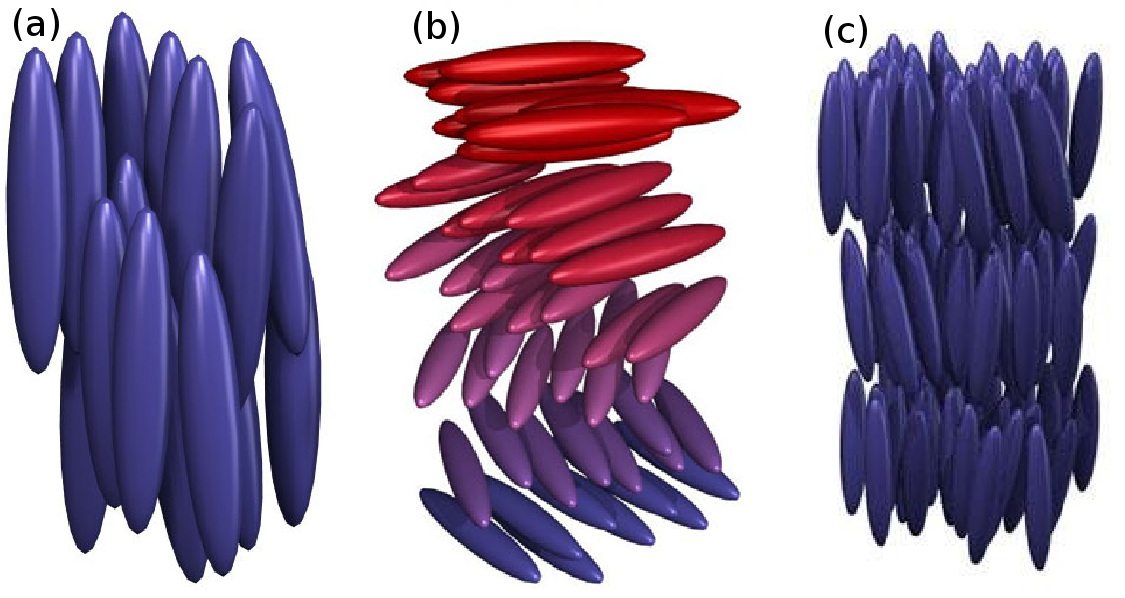
\includegraphics[width=.8\textwidth]{faze}
 \caption{Shematski prikaz treh najpogostej"sih teko"cekristalnih mezofaz: (a) nematik, (b) kiralni nematik ali holesterik in (c) smektik \cite{barrett:lc}.}
  \label{fig:faze}
\end{figure}

\section{Orientacijski red}

V vseh teko"cekristalnih mezofazah imajo gradniki orientacijski red dolgega dosega. 
Definiramo lahko enotski vektor $\mathbf{n}$, ki dolo"ca povpre"cno smer gradnikov in ga imenujemo direktor. 
Direktor ni pravi vektor, saj v teko"cem kristalu ne lo"cimo med smerjo $\mathbf{n}$ in $\mathbf{-n}$. 
Tudi "ce sami gradniki nimajo tak"sne simetrije, jo imajo njihove fluktuacije \cite{mermin}. 

\begin{figure}[h]
\begin{center}
\subfigure{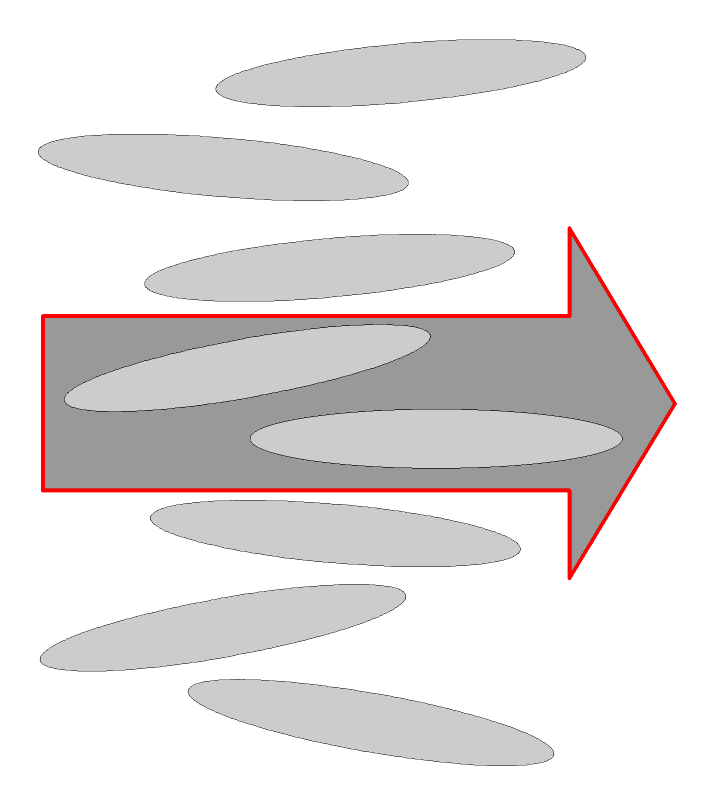
\includegraphics[height=100pt]{Nematic-Director}}
\subfigure{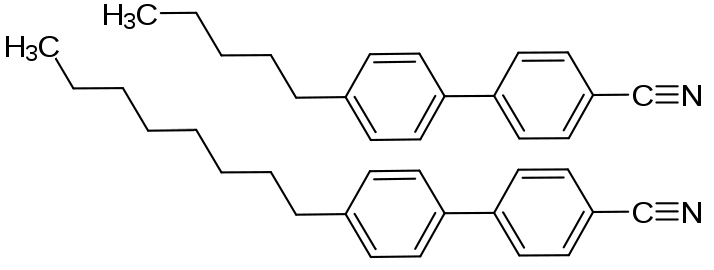
\includegraphics[height=100pt]{nematik-formuli}}
 \caption{Levo: Gradniki imajo razli"cne orientacije, preferen"cno smer pa poda direktor. Desno: Strukturni formuli molekul 5CB (zgoraj) in 8CB (spodaj) \cite{wiki:lc}}
 \label{fig:nematik-direktor}
 \end{center}
\end{figure}

Orientacijski red dolgega dosega je tipi"cno realiziran s pali"castimi gradniki. 
Najpogosteje se uporabljajo organske molekule z dvema benzenovima obro"cema, na katera so vezane razli"cne skupine. 
Primera tak"snih molekul sta 4-ciano-4'-pentilbifenil (5CB) in 4-ciano-4'-oktilbifenil (8CB), katerih strukturni formuli sta prikazani na Sliki \ref{fig:nematik-direktor}. 
Tipi"cna dol"zina tak"snih molekul je nekaj nanometrov. 

Direktor $\mathbf{n}$ podaja povpre"cno smer gradnikov, ne pa dejanske orientacije posameznih gradnikov, t.i. molekularnih direktrojev. 
Zato uvedemo "se stopnjo reda $S$ \angl{degree of order}, ki nam pove, koliko smeri molekul v povpre"cju odstopajo od direktorja. 
Zaradi simetrije $\mathbf{n} \leftrightarrow -\mathbf{n}$ ne moremo vzeti kar povpre"cne vrednosti kota med gradnikom in direktorjem, saj je ta vrednost enaka ni"c. 
Namesto tega uporabimo povpre"cni kvadrat kota, ki je ekvivalenten kvadrupolnemu momentu \cite{kleman}
\begin{align}
 S = \frac{1}{2}\left(3\langle\cos^2\vartheta\rangle-1\right),
\end{align}
kjer je $\vartheta$ kot med osjo gradnika in direktorjem, $\langle\rangle$ pa ansambelsko ali "casovno povpre"cje. 
Pri tak"sni definiciji ima popolnoma urejen teko"ci kristal, kjer so vsi gradniki vzporedni z direktorjem, vrednost $S=1$, povsem neurejen teko"ci kristal z naklju"cnimi orientacijami molekul pa $S=0$. 
V Landauovi teoriji faznih prehodov je ureditveni parameter koli"cina, ki je v eni fazi tipi"cno enaka ni"c, v drugi pa od ni"c razli"cna. 
Zgoraj definirana stopnja reda $S$ je tako primeren ureditveni parameter za opis prehoda med izotropno teko"cino in teko"cekristalno fazo \cite{degennes}. 

Direktor in nematsko stopnjo reda lahko hkrati opi"semo z eno tenzorsko koli"cino. V ta namen uvedemo tenzor ureditvenih parametrov $Q_{ij}$ kot
\begin{align}
  Q_{ij} = \frac{S}{2}(3n_i n_j - \delta_{ij}) + \frac{P}{2}(e^{(1)}_i e^{(1)}_j - e^{(2)}_i e^{(2)}_j)\,,
\end{align}
kjer sta $\mathbf{e}^{(1)}$ in $\mathbf{e}^{(2)}$ enotska vektorja, pravokotna na $\mathbf{n}$ in med seboj. 
Uvedli smo "se biaksialnost $P$, ki je neni"celna, "ce fluktuacije molekul niso simetri"cne na vrtenje okrog direktorja. 
V tem primeru imamo orientacijski red tudi vzdol"z osi $e^{(1)}$, ki je pravokotna na direktor in jo imenujemo sekundarni direktor. 
Parameter $P$ ima podoben pomen kot $S$ in nam pove, kako dobro so gradniki urejeni glede na sekundarni direktor. 
Ker komponente $n_i$ nastopajo le v kvadratu, s tak"snim zapisom avtomatsko upo"stevamo simetrijo direktorja, saj zamenjava $\mathbf{n}$ z $-\mathbf{n}$ tenzorja $Q_{ij}$ ne spremeni. 
Ker je $\mathbf{n}$ enotski vektor, je tenzor $Q_{ij}$ brezsleden, zato so v izotropni snovi vse njegove komponente enake 0 in je primeren ureditveni parameter za opis faznih prehodov. 

Tenzor ureditvenih parametrov $Q_{ij}$ lahko v vsaki to"cki predstavimo kot matriko velikosti $3\times 3$, ki je simetri"cna in zato diagonalizabilna. 
V lastnem sistemu direktorja, kjer za osi koordinatnega sistema vzamemo $\vec n$, $\vec e^{(1)}$ in $\vec e^{(2)}$, lahko matriko zapi"semo kot

\begin{equation}
 Q = \begin{pmatrix}
  S &   & \\
  & \frac{-S+P}{2} & \\
  & & \frac{-S-P}{2}
 \end{pmatrix}
\end{equation}

S tak"snim zapisom je razvidno, kako lahko iz podanega tenzorja $Q_{ij}$ izra"cunamo direktor $\vec n$ in stopnjo reda $S$. 
Stopnja reda je enaka najve"cji lastni vrednosti matrike $Q$, direktor pa je lastni vektor, ki ustreza tej lastni vrednosti. 
Ra"cun lastnih vektorjev ne lo"ci med vektorji, ki se razlikujejo le za predznak, tako da na ta na"cin zadostimo simetriji direktorja. 

\section{Deformacije direktorja in prosta energija}

Ureditev teko"cega kristala lahko opi"semo s tenzorskim poljem $Q_{ij}(\vec r)$, ki podaja tenzor ureditvenih parametrov v vsaki to"cki. 
Skupno prosto energijo lahko izrazimo kot funkcional polja $Q_{ij}(\vec r)$, ki pa je odvisen od teko"cekristalne mezofaze. 
V tej nalogi obravnavamo le nematsko mezofazo, ki je najpogostej"sa in najbolj enostavna. 
K prosti energiji nematika prispevajo elasti"cne deformacije, stopnja reda in dielektri"cna interakcija z elektri"cnim poljem. 
Drugi prispevki, npr. magnetna interakcija in fleksoelektri"cnost, so pri obi"cajno uporabljanih snoveh in opti"cnem polju zanemarljivi.

\begin{figure}[h]
\begin{center}
  \begin{picture}(400, 120)
    \put(0,30){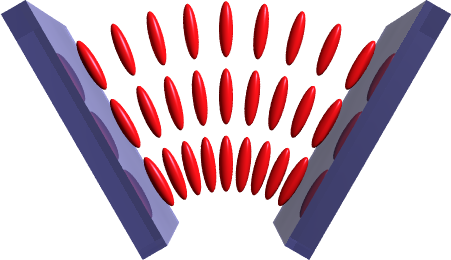
\includegraphics[height=80pt]{fig_frank_components_splay_s}}
    \put(150,20){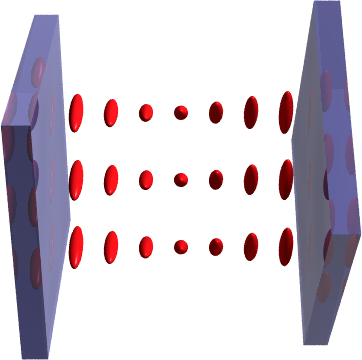
\includegraphics[height=100pt]{fig_frank_components_twist_s}}
    \put(270,30){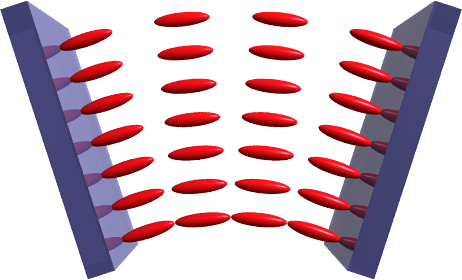
\includegraphics[height=80pt]{fig_frank_components_bend_s}}
    \put(20, 110){(a)}
    \put(170, 110){(b)}
    \put(290, 110){(c)}
    \put(45, 10){$\nabla \cdot \vec n \neq 0$}
    \put(165, 10){$\vec n \cdot \nabla \times \vec n \neq 0$}
    \put(300, 10){$\vec n \times \nabla \times \vec n \neq 0$}
  \end{picture}
  \caption{Trije na"cini elasti"cne deformacije direktorja: (a) pahlja"ca, (b) zvoj in (c) upogib \cite{copar-phd}. }
\label{fig:tsb}
\end{center}
\end{figure}
Posamezni gradniki imajo najve"cjo svobodo gibanja in s tem najve"cjo entropijo, "ce je direktor in s tem tudi teznor $Q_{ij}$ uniformen. 
Krajevno spreminjanje ureditvenega parametra $Q_{ij}$ v katerikoli smeri povzro"ci, da sistemu prosta energija naraste. 
To pove"canje je odvisno od smeri spreminjanja $Q_{ij}$ glede na smer direktorja. 
Na sliki \ref{fig:tsb} so prikazani trije na"cini deformacije direktorja, s katerimi lahko lokalno opi"semo poljubno krajevno odvisnost. 
Ti trije na"cini so pahlja"ca \angl{splay}, zvoj \angl{twist} in upogib \angl{bend}. 

\todo{Mapping med na"cini deformacije in odvodi direktorja}

Vsi trije na"cini deformacije so elasti"cni, zato je prispevek v prosti energiji sorazmeren s kvadratom deformacije. 
V teko"cih kristalih so v splo"snem elasti"cne konstante, ki pripadajo vsakemu izmed treh osnovnih na"cinom, med seboj razli"cne. 
Prispevek k gostoti proste energije zaradi elasti"cnih deformacij nematskega teko"cega kristala je tako enak
\begin{align}
 f_{\mathrm{el}}^N &= \frac{K_1}{2} (\nabla \cdot \vec n)^2 + \frac{K_2}{2} (\vec n \cdot \nabla \times \vec n)^2 + \frac{K_3}{2} (\vec n \times \nabla \times \vec n)^2. 
\end{align}

Tri elasti"cne konstante $K_i$ so v splo"snem razli"cne. Tipi"cno je konstanta $K_3$, ki ustreza upogibni deformaciji, mnogo ve"cja od ostalih dveh, konstanta $K_2$, ki ustreza zvoju, pa malo manj"sa od $K_1$. 
Kljub temu pa so v ve"cini nematikov vse tri konstante istega velikostnega reda \cite{degennes}. 
Modeliranje teko"cega kristala lahko poenostavimo, "ce privzamemo, da so vse tri konstante enake. 
V t. i. enokonstantnem pribli"zku je gostota elasti"cne proste energije enaka
\begin{align}
 f_{\mathrm{el}} &= \frac{K}{2} \left[(\nabla \cdot \vec n)^2 + (\nabla \times \vec n)^2\right] = \frac{K}{2} \cdot \nodv{i}{j}\nodv{j}{i}
\end{align}
kjer je $K$ edina elasti"cna konstanta.
Razvoj elasti"cne proste energije po krajevnih odvodih direktorja je la"zji za predstavo, saj "clene lahko pove"zemo z na"cini deformacije na sliki \ref{fig:tsb}. 
Za numeri"cno modeliranje pa je bolj ugodno, "ce jo izrazimo s komponentami tenzorja $Q$, ki poleg direktorja vklju"cuje tudi stopnjo reda in dvoosnost \cite{copar-phd}. 
V tej sliki se izraz glasi
\begin{align}
 f_{\mathrm{el}} &= \frac{1}{2}L_1\qodv{ij}{k}\qodv{ij}{k} + \frac{1}{2}L_2 \qodv{ij}{j}\qodv{ik}{k} + \frac{L_3}{2}Q_{ij}\qodv{kl}{i}\qodv{kl}{j}\;,
\end{align}
kjer so $L_i$ elasti"cne konstante. V enokonstantnem pribli"zku se zgornji izraz poenostavi v 
\begin{align}
f_{\mathrm{el}} &= \frac{L}{2} \times \qodv{ij}{k}\qodv{ij}{k} 
\end{align}
kjer je elasti"cna konstanta enaka $L = 2K/9S^2$ \cite{ravnik-zumer-ldg}. 

Stabilnost nematske mezofaze je odvisna od temperature ali od koncentracije. 
Za termotropske teko"ce kristale, kjer je mezofaza odvisna od temperature, lahko zapi"semo Landauov razvoj proste energije po ureditvenem parametru $Q_{ij}$ kot
\begin{align}
  f_{\mathrm{L}} = \frac{1}{2}a(T-T^\ast)Q_{ij}Q_{ji} + \frac{1}{3}BQ_{ij}Q_{jk}Q_{ki} + \frac{1}{4}C(Q_{ij}Q_{ji})^2,
\end{align}
kjer je $T$ temperatura, $T^\ast$ najni"zja mo"zna temperatura podhlajene izotropne faze, $a$, $B$ in $C$ pa "cleni Landauovega razvoja in so odvisni od snovi. 
Zaradi definicije stopnje reda stanji s $S$ in $-S$ nista enakovredni, zato v razvoju nastopa tudi "clen tretjega reda v $S$ oz. v $Q_{ij}$ \cite{degennes,ravnik-zumer-ldg}. 

Ker sta konstanti $a$ in $C$ pozitivni, je pri temperaturi nad $T^\ast$ najugodnej"se stanje $Q_{ij}=0$ oz. $S=0$, kar ustreza izotropni snovi. 
Pri temperaturi pod $T^\ast$ pa kvadratni "clen zamenja predznak, zaradi "cesar postane stabilno tudi stanje z neni"celnim ureditvenim parametrom, torej nematska mezofaza. 

Na ureditev pa vpliva tudi zunanje elektri"cno polje. 
Prispevek k prosti energiji lahko razdelimo na prispevek izotropnega dela dielektri"cnega tenzorja $\overline\varepsilon$, ki ni odvisen od ureditve teko"cega kristala, in prispevka dielektri"cne anizotropije, ki predstavlja sklopitev med ureditvijo in elektri"cnim poljem. 
Skupna sprememba proste energije je enaka
\begin{align}
\label{eq:dielektricna-sklopitev}
  f_{\mathrm{EM}} = -\frac{1}{2}\varepsilon_0 \left(\overline\varepsilon E_i E_i + \frac{2}{3}\varepsilon_a^{\mathrm{mol}} E_iQ_{ij}E_j \right),
\end{align}
kjer je $\overline{\varepsilon}$ povpre"cna dielektri"cna konstanta, $\varepsilon_a^{\mathrm{mol}} = \varepsilon_{\parallel}^{\mathrm{mol}} - \varepsilon_{\perp}^{\mathrm{mol}}$ dielektri"cna anizotropija posamezne molekule, $E_i$ pa zunanje elektri"cno polje. 
Ta sklopitev izhaja iz polarizabilnosti molekul, ki je odvisna od njihove oblike. 
V snovi s pozitivno dielektri"cno anizotropijo je najugodnj"sa 
Zunanje polje v molekuli inducira elektri"cni dipolni moment, ki je sorazmeren z dol"zino molekule in je zato najve"cji, "ce je polje vzporedno z osjo molekule. 


Tipi"cen relaksacijski "cas lahko ocenimo s primerjavo viskoznosti ter elasti"cne in dielektri"cne proste energije
\begin{align}
 \frac{1}{\tau} \sim \frac{f_\mathrm{el} + f_\mathrm{EM}}{\gamma_1}\,.
\end{align}
Ker nas zanima le red velikosti, lahko uporabimo enokonstantni pribli"zek, krajevni odvod direktorja pa zamenjamo z obratno vrednostjo dol"zinske skale $l$, na kateri se direktor spreminja. 
Ta dol"znina je tipi"cno velikostnega reda mikrometra \cite{kleman}. 
V elektri"cnem prispevku za oceno velikostnega reda privzamemo popolnoma urejen nematik in elektri"cno polje, vzporedno z direktorjem. 
S temi predpostavkami lahko ocenimo relaksacijski "cas teko"cega kristala v elektri"cnem polju
\begin{align}
% za v KRunner: 0.06 Pas / (6*10^(-12)N / (1um)^2 + 8.86*10^(-12) As/Vm * 0.5 * (3V/um)^2 ) =
 \tau \sim \frac{\gamma_1}{K/l^2 + \varepsilon_0 \varepsilon_a^{\mathrm{mol}} E^2 } \sim 1\;\mathrm{ms}\,.
\end{align}
kjer je $\gamma_1$ rotacijska viskoznost. 
Pri vrednosti viskoznosti $\gamma_1 \approx 0,\!06 \; \mathrm{Pa\,s}$, elasti"cne konstante $K \approx 6\times 10^{-12} \; \mathrm{N}$ in dielektri"cne anizotropije $\varepsilon_a^{\mathrm{mol}} \approx 0,\!4$ za 5CB \cite{diploma-miha,kolicniki} in jakosti elektri"cnega polja $E = 1\mathrm{V}/\mu\mathrm{m}$, tipi"cni za opti"cne pincete, relaksacijski "cas zna"sa pribli"zno 1 ms. 
Ta vrednost je odvisna od jakosti elektri"cnega polja, ampak preureditev teko"cega kristala je tudi pri zelo mo"cnem polju ve"c velikostnih redov po"casnej"sa od nihanja opti"cnega polja s periodo velikostnega reda femtosekunde. 
"Ce na teko"ci kristal svetimo, ureditev molekul ne more slediti hitremu spreminjanju opti"cnega elektri"cnega polja, ampak nanj efektivno deluje povpre"cen kvadrat polja. 

\section{Topolo"ski defekti}

Pod vplivom ograjenosti ali zunanjega polja se lahko v nematiku pojavi orientacijsko polje, kjer zvezno direktorsko polje ne more zadostiti robnim pogojem. 
V tem primeru se pojavijo obmo"cja z nedifiniranim direktorjem. 
Tak"snim obmo"cjem pravimo topolo"ski defekti. 

V treh dimenzijah lahko obstajajo to"ckasti in linijski defekti \cite{degennes,kleman}. 
V vlaknih nastopajo le linijski defekti, imenovani tudi disklinacije, zato se bomo posvetili zlasti tistim. 
Linijski defekti so la"zji za razvr"s"canje, saj se lahko omejimo na ravnino, pravokotno na linijo, in problem prevedemo na dve dimenziji. 
V tem primeru lahko praviloma linijski defekt obravnavamo kot to"ckasti defekt v dveh dimenzijah. 

Disklinacije v nematskem teko"cem kristalu delimo glede na to, kako se smer direktorja spreminja v okolici disklinacije. 
Zanima nas zlasti, koliko obratov naredi direktorsko polje, "ce defekt obkro"zimo po zaklju"ceni zanki. 
V dveh dimenzijah lahko nematski direktor zapi"semo kot $\vec n = (\cos\theta, \sin\theta, 0)$. 
Definiramo lahko ovojno "stevilo \angl{winding number} oz. mo"c defekta kot
\begin{align}
\label{eq:winding-number}
 s = \frac{1}{2\pi}\int_0^{2\pi} \left(\frac{d\theta}{d\phi}\right) \dd \phi
\end{align}
kjer kot $\theta$ opisuje smer direktorja, $\phi$ pa polo"zaj na zanki (svetlo modra na slikah \ref{fig:defekti-celi} in \ref{fig:defekti-polceli}). 

Direktorsko polje je zvezno povsod razen v jedru defekta, zato mora direktor pri $\phi = 0$ enak kot pri $\phi = 2\pi$, seveda ko upo"stevamo se simetrijo $\vec n \leftrightarrow -\vec n$.
Ta pogoj dolo"ca mo"zne vrednosti za $s$. 
Za prava vektorska polja mora biti $s$ celo "stevilo, saj mora biti kot $\theta$ na koncu enak kot na za"cetku. 
Primeri tak"snih defektov so na sliki \ref{fig:defekti-celi}. 

\begin{figure}[h]
 \centering
 \subfigure{\includegraphics[height=100pt]{g_defect_-4}}
 \subfigure{\includegraphics[height=100pt]{g_defect_-2}}
 \subfigure{\includegraphics[height=100pt]{g_defect_2}}
 \subfigure{\includegraphics[height=100pt]{g_defect_4}}
 \caption{Linijski defekti s celo"stevilosko mo"cjo. Mo"c defekta je odvisna od tega, kolikokrat se zavrti direktor (temno modre "crte), ko naredimo en krog po svetlo modrem krogu. Od leve proti desni so mo"ci $-2$, $-1$, $1$ in $2$. }
 \label{fig:defekti-celi}
\end{figure}

Nematski direktor pa ima dodatno simetrijo, zaradi katere lahko direktor pri obkro"zenju defekta naredi le pol obrata, ovojno "stevilo $s$ pa je zato lahko tudi polcelo "stevilo. 
Primeri tak"snih defektov so na sliki \ref{fig:defekti-polceli}. 

\begin{figure}[h]
 \centering
 \subfigure{\includegraphics[height=100pt]{g_defect_-3}}
 \subfigure{\includegraphics[height=100pt]{g_defect_-1}}
 \subfigure{\includegraphics[height=100pt]{g_defect_1}}
 \subfigure{\includegraphics[height=100pt]{g_defect_3}}
 \caption{Linijskih defekti s polcelo mo"cjo. Polcele vrednosti so mo"zne zaradi simetrije direktorja. Od leve proti desni so mo"ci $-3/2$, $-1/2$, $1/2$ in $3/2$. }
 \label{fig:defekti-polceli}
\end{figure}

Vsi defekti z enakim ovojnim "stevilom so si topolo"sko ekvivalentni, saj lahko enega zvezno transformiramo v drugega. 
Mo"ci defekta pravimo tudi topolo"ska invarianta, saj se defekti lahko zdru"zujejo in pretvarjajo eden v drugega, skupen topolo"ski naboj pa se ohranja. 
Dva defekta z nasprotno mo"cjo se lahko izni"cita, defekt z ve"cjo mo"cjo pa se lahko razcepi na dva defekta z manj"so mo"cjo. 
Pri tem velja omejitev, da je mo"c vsakega defekta lahko le polcelo "stevilo. 

Vsak defekt v teko"cem kristalu povzro"ci elasti"cno deformacijo direktorskega polja, kar pomeni lokalno veliko gostoto proste energije na mestu defekta. 
Za linijske defekte v enokonstantnem pribli"zku je gostota elasti"cna proste energije enaka $\frac{K}{2}(\nabla \theta)^2$. 
V bli"zini defekta lahko privzamemo odvisnost $\theta(\phi) = s \phi + \theta_0$, iz "cesar sledi $\nabla\theta = \frac{s}{r}\hat e_\phi$. 
Skupni prispevek enega defekta k prosti energiji na enoto dol"zine $l$ je enak \cite{degennes}
\begin{align}
 \frac{F_d}{l} &= \frac{K}{2} \int_{r_{min}}^{r_{max}} \frac{s^2}{r^2} 2\pi r \dd r = K s^2 \pi \ln{\frac{r_{max}}{r_{min}}}
\end{align}
Zgornji izraz divergira tako v bli"zini defekta kot tudi za velike oddaljenosti. 
Velikostna skala $r_{max}$ je povezana z velikostjo sistema oz. z razdaljo do sosednjega defekta. 
En sam izoliran defekt ni stabilen, razen "ce ga vsiljujejo robni pogoji. 
Jedro defekta se pogosto obravnava kot obmo"cje izotropne faze z S=0.
Velikost staljenega dela opisuje $r_{min}$ in je tipi"cno okrog 10 nm. 

V zgornji enakosti je pomembna odvisnost od ovojnega "stevila. 
Elasti"cna energija zaradi defekta je sorazmerna z $s^2$, zato je bolj ugodno, da se defekt z ve"cjim ovojnim "stevilom razcepi na ve"c manj"sih defektov. 
Stabilni defekti so le tisti z ovojnim "stevilom $s=\pm1/2$, vsi ostali razpadejo na ve"c defektov z manj"sim nabojem. 

\section{Direktor v cilindri"cni kapilari}

V cilindri"cni geometriji s homeotropnimi robnimi pogoji ureditev z uniformnim direktorjem ni mo"zna. 
Glede na razmerja med elasti"cnimi konstantami se teko"ci kristal uredi v eno izmed konfiguracij na sliki \ref{fig:director-profiles}. 
V profilu s singularno disklinacijo v osi kapilare je prisotna le pahlja"cna deformacija, zato je energija tega stanja odvisna od konstante $K_1$. 
V pobeglem profilu pa sta prisotni tako pahlja"cna kot upogibna deformacija.
Energija tega stanja je odvisna od konstant $K_1$ in $K_3$. 
Do pobega pride, "ce je razmerje $K_3/K_1$ manj"se od 13 \cite{kleman}, kar velja za ve"cino nematskih teko"cih kristalov. 
Z minimizacijo energije lahko izpeljemo ravnovesni radialni profil direktorja v cilindri"cnih koordinatah. 
V poenostavljenem primeru, ko sta elasti"cni konstanti $K_3$ in $K_1$ enaki, je energijsko najugodneje"se stanje 
\begin{align}
 \vec n &= (n_r, n_\phi, n_z) = (\cos \chi(r), 0, \sin \chi(r)) \\
 \chi(r) &= 2 \arctan \frac{R-r}{R+r}
\end{align}
kjer je $R$ polmer kapilare. 
Tak"sen profil je prikazan na sliki \ref{fig:director-profiles}b. 
V primeru pobega v tretjo dimenzijo je direktor povsod dobro definiran. 
"Ce pa do pobega ne pride, je tik ob osi kapilare defekt. Okrog defekta je direktorsko polje radialno, torej je to linijski defekt z ovojnim "stevilom $s=+1$. 

\begin{figure}[!htbp]
\centering
\subfigure{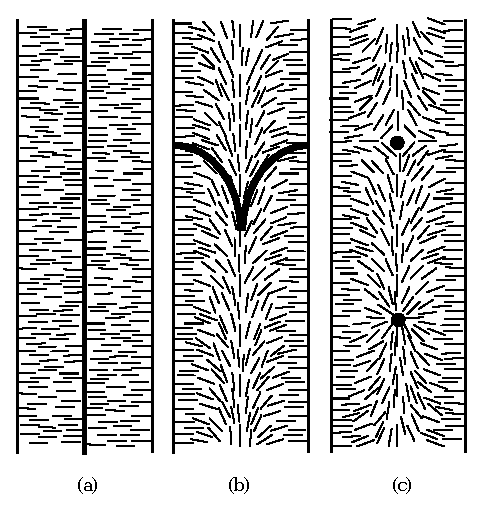
\includegraphics[height=150px]{director-profile-cylinder-kleman}}
\subfigure{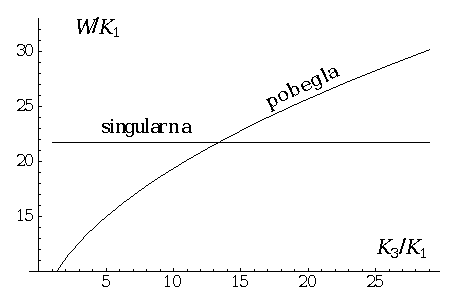
\includegraphics[clip, trim=0cm -3mm 0cm 0cm]{escaped-director-energy}}
\caption{Levo: Prerezi kapilare s singularno (a) in nesingularno pobeglo defektno linijo (b). 
Razli"cne smeri pobega povzro"cijo nastanek to"ckastih defektov (c). Desno: Energija singularne in pobegle konfiguracije v odvisnosti od razmerja med elasti"cnima kostantama $K_1$ in $K_3$ \cite{kleman}. }
 \label{fig:director-profiles}
\end{figure}

V ve"cini nematikov so vse tri elasti"cne konstante istega velikostnega reda, zato je stanje s pobegom v tretjo dimenzijo bolj ugodno. 
Veliko razmerje $K_3/K_1$ pa opazimo blizu faznega prehoda v smekti"cno fazo. 

Z uporabo 8CB, ki tvori tako nematsko kot tudi smekti"cno fazo, je mogo"ce v laboratoriju sintetizirati vlakna z radialnim profilom direktorja \cite{peddireddy}. 
\todo{Napisi, kako to naredijo}
Primer tvorbe tak"snih vlaken je na sliki \ref{fig:tvorjenje}. 

\begin{figure}[h]
 \centering
 \subfigure{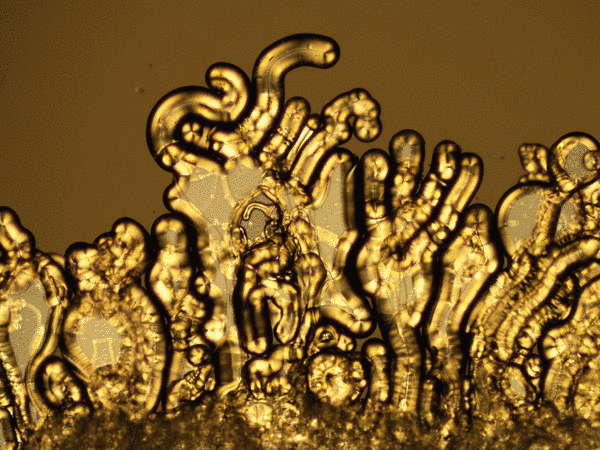
\includegraphics[height=150px]{tvorjenje}}
 \subfigure{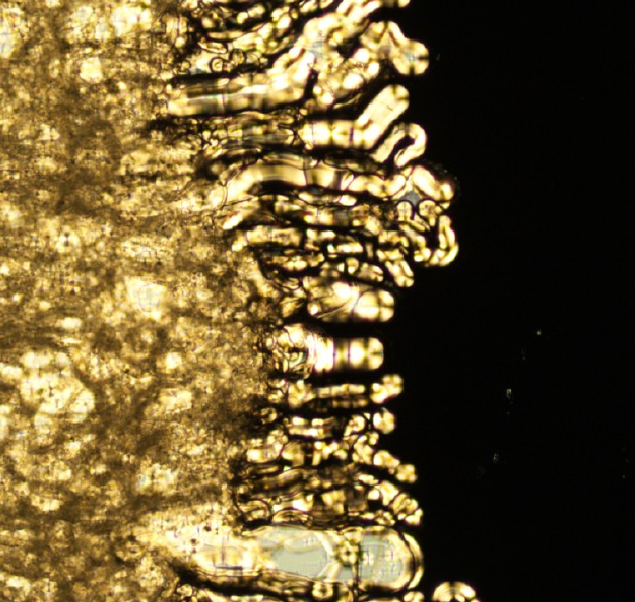
\includegraphics[height=150px]{tvorjenje2}}
 \caption{Rast vlaken z radialnim direktorjem na meji med teko"cim kristalom 8CB in vodo \cite{peddireddy}}
 \label{fig:tvorjenje}
\end{figure}

\chapter{Elektromagnetno valovanje}

\section{Maxwellove ena"cbe v opti"cno anizotropnem mediju}
"Sirjenje svetlobe po snovi opisujejo "stiri Maxwellove ena"cbe \cite{taflove}
\begin{equation}
\begin{aligned}
 \nabla \cdot \vec D = \rho_f & \qquad \nabla \cdot \vec B = 0 \\
 \nabla \times \vec E = -\odvod{\vec B}{t} & \qquad \nabla \times \vec H = \vec J_f + \odvod{\vec D}{t}
\end{aligned} 
\end{equation}
kjer sta $\vec E$ in $\vec D$ jakost in gostota elektri"cnega polja, $\vec H$ in $\vec B$ pa jakost in gostota magnetnega polja. 
Med njimi veljata konstitutivni zvezi $\vec D = \varepsilon \varepsilon_0 \vec E$ in $\vec B = \mu \mu_0 \vec H$. 
V ena"cbah nastopata izvora elektromagnetn	ih polj, in sicer gostota prostih nabojev $\rho_f$ in gostota prostega toka $J_f$. 

V teko"cih kristalih sta dielektri"cnost $\varepsilon$ in permeabilnost $\mu$ anizotropna tenzorja. 
Obi"cajno je pri opti"cnih frekvencah magnetna anizotropija mnogo "sibkej"sa od elektri"cne, zato jo lahko zanemarimo in privzamemo $\mu = 1$. 

Izvori in ponori valovanja znotraj vzorca so posledica neni"celne elektri"cne prevodnosti materiala.
Zaradi prevodnosti $\sigma$ ob prisotnosti elektri"cnega polja v snovi te"ce tok, ki je enak $\vec J = \sigma \vec E$. 
Prostih nabojev tipcno v tekocekristlaih sistemih ni, zato je $\rho_f=0$. 
Z upo"stevanjem zgornjih predpostavk lahko Maxwellove ena"cbe zapi"semo v poenostavljeni obliki
\begin{equation}
  \begin{aligned}
  \nabla \cdot \vec E = 0 & \qquad \nabla \cdot \vec B = 0 \\
  \nabla \times \vec E = -\odvod{\vec B}{t} & \qquad \nabla \times \vec B = \sigma \vec E + \varepsilon\varepsilon_0\mu_0\odvod{\vec E}{t}
  \end{aligned}
\end{equation}
V zadnji ena"cbi smo privzeli, da se dielektri"cni tenzor $\varepsilon$ ne spreminja s "casom, zato nastopa izven "casovnega odvoda. 
Ta predpostavka je smiselna pri obravnavi opti"cnih polj, saj je relaksacija teko"cega kristala mnogo po"casnej"sa od sprememb elektri"cnega in magnetnega polja. 
V tipi"cnem teko"cem kristalu in frekvencah vidne svetlobe je razlika v "casovni skali okrog 15 redov velikosti. 

\section{Dvolomnost}
Dvolomnost \angl{birefringence} je pojav, pri katerem je lomni koli"cnik snovi odvisen od polarizacije svetlobe \cite{landau-lifsic-optics, wiki:birefringence}. 
Opazimo jo predvsem pri kristalih, kot sta kalcit in vodni led, pa tudi nekaterih vrstah plastike. 
Lahko je posledica same strukture snovi, na primer pri kristalih, oblike gradnikov kot pri teko"cih kristalih, ali pa jo vsilimo z mehansko obremenitvijo. 

V dvolomnih snoveh zveze med jakostjo elektri"cnega polja $E$ in gostoto elektri"cnega polja $D$ ne moremo opisati s skalarjem, ampak s tenzorjem
\begin{align}
  D_i &= \varepsilon_0 \varepsilon_{ij} E_j
\end{align}

Dielektri"cni tenzor $\varepsilon_{ij}$ je linearna zveza med dvema vektorskima koli"cinama. 
Predstavimo ga z matriko velikosti $3\times 3$, torej ima tri lastne smeri in tri lastne vrednosti.
Najenostavnej"sa in najpogostej"sa vrsta dvolomnosti je tak"sna, pri katerem sta dve izmed lastnih vrednosti enaki, tretja je pa razli"cna. 
Lastni smeri, ki ustreza razli"cni lastni vrednosti, pravimo opti"cna os. 
V tak"sni snovi je le ena privilegirana os, zato re"cemo, da je snov opti"cno enoosna. 
V lastnem sistemu lahko tenzor zapi"semo kot
\begin{align}
  \varepsilon = \begin{pmatrix}\varepsilon_\perp & & \\ & \varepsilon_\perp & \\ & & \varepsilon_\parallel \end{pmatrix}
\end{align}
Tu je $\varepsilon_\parallel$ lastna vrednost, ki ustreza polarizaciji svetlobe, vzporedni z opti"cno osjo. 
Tej polarizaciji pravimo izredna \angl{extraordinary}, ustreznemo lomnemu koli"cniku $n_e = \sqrt{\varepsilon_\parallel}$ pa izredni lomni koli"cnik. 
Polarizacija svetlobe, pravokotna na opti"cno os je redna \angl{ordinary}, ustreza pa ji redni lomni koli"cnik $n_o = \sqrt{\varepsilon_\perp}$. 
Dvolomnost snovi lahko kvantitativno opi"semo z razliko med izrednim in rednim lomnim koli"cnikom
\begin{align}
  \Delta n = n_e - n_o\;,
\end{align}
ki je lahko pozitivna ali negativna. 

\begin{figure}[h]
  \centering
  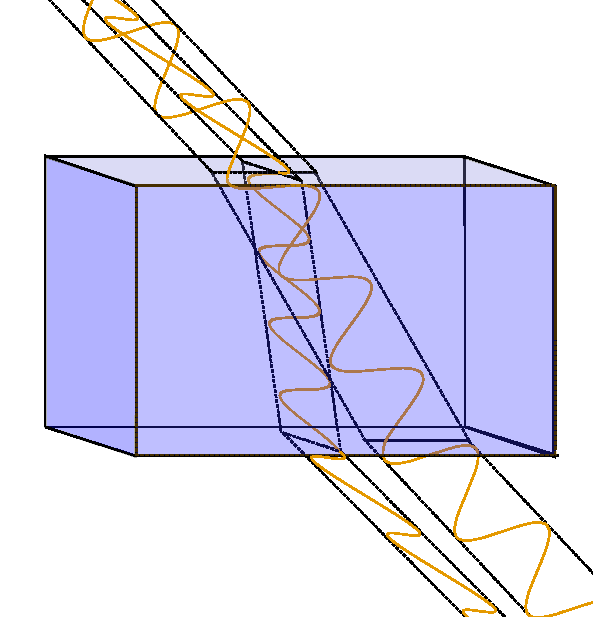
\includegraphics[height=150pt]{Rays_passing_through_birefringent_material}
  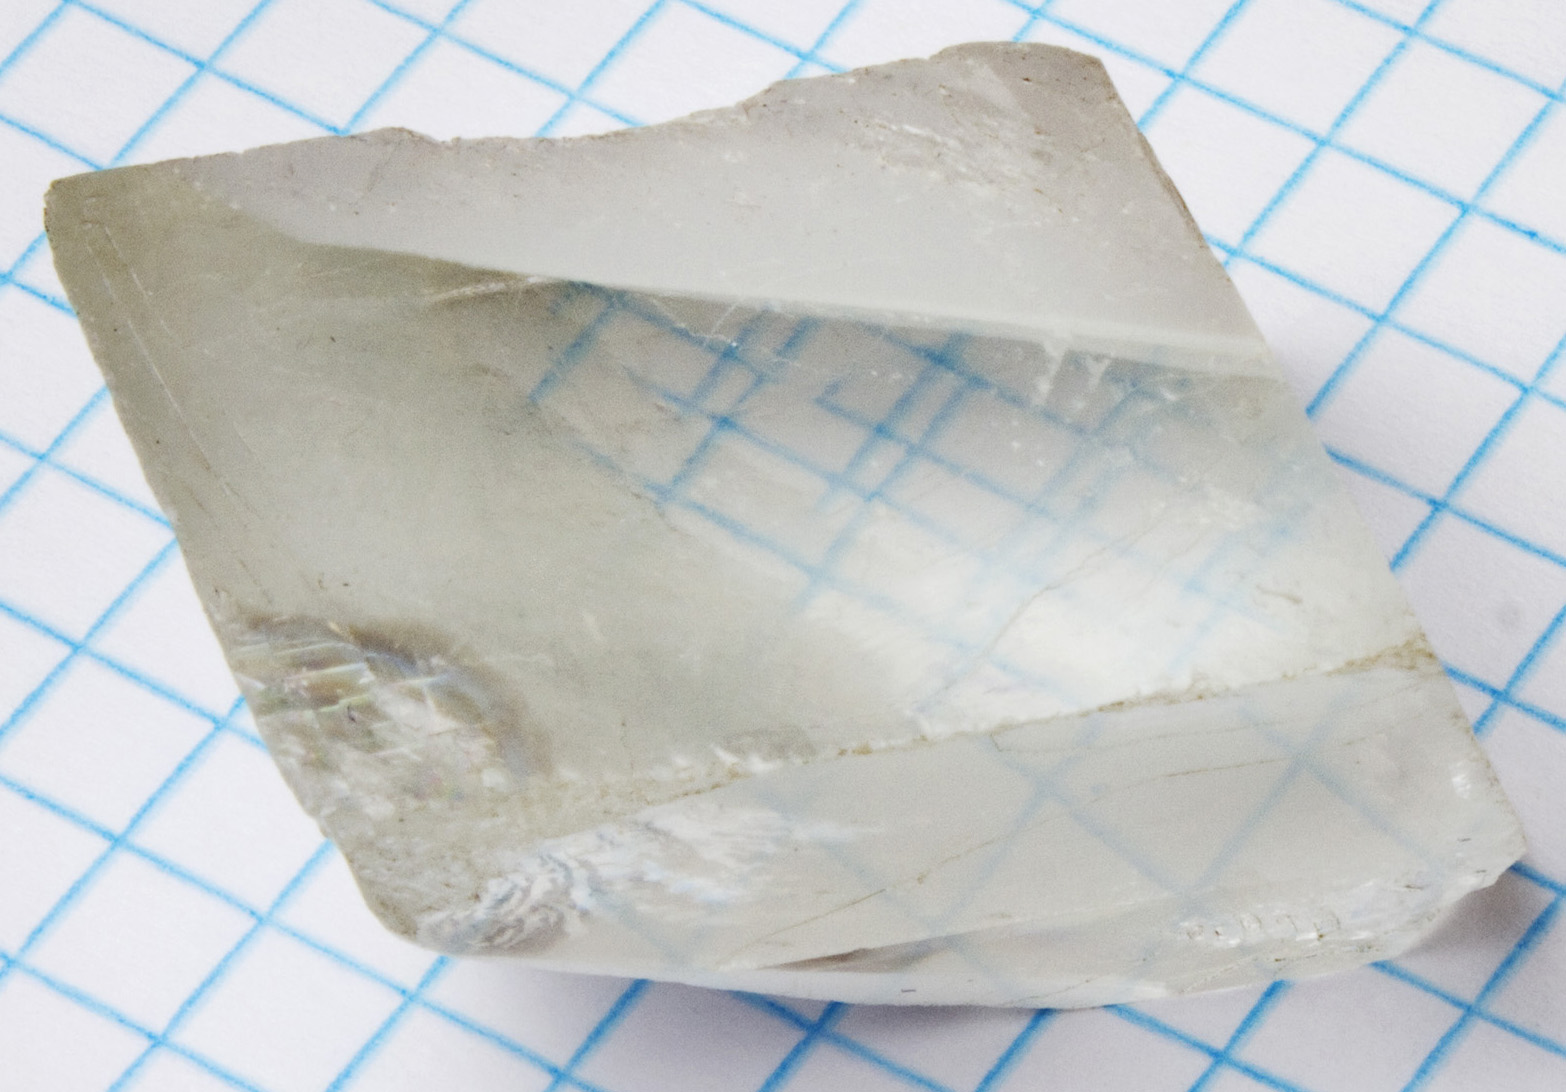
\includegraphics[height=150pt]{Crystal_on_graph_paper}
  \caption{Levo: Prehod svetlobnih "zarkov z razli"cnima polarizacijama skozi dvolomno snov. 
Zaradi razli"cnih polarizacij se "zarka razli"cno lomita. Desno: Pogled skozi dvolomni kristal kalcita. Vidni sta dve sliki vzorca pod kristalom. \cite{wiki:birefringence}}
  \label{fig:dvolomnost}
\end{figure}

Enako kot dielektri"cnost $\varepsilon$ lahko tudi anizotropna magnetna permeabilnost $\mu$ povzro"ci dvolomnost. 
Pri opti"cnih frekvencah je magnetna anizotropija ve"cine snovi zanemarljiva, zato je dovolj obravnavati le elektri"cno. 

Hitrost svetlobe v tak"sni snovi je enaka
\begin{align}
  c &= \sqrt{\frac{1}{\varepsilon_{\mathrm{eff}} \varepsilon_0 \mu_0}} = \frac{c_0}{\sqrt{\varepsilon_{\mathrm{eff}}}} = c_0\sqrt{\frac{E_iE_i}{E_i \varepsilon_{ij} E_j}}
\end{align}
in je odvisna od smeri elektri"cnega polja. 

\section{Defekti v polarizaciji svetlobe}
Elektri"cno in magnetno polje sta prava vektorja, zato imata lahko le defekte s celo"stevilskim ovojnim "stevilom. 
Defekt v elektromagnetnem polju je to"cka oz. obmo"cje, kjer polarizacija in faza valovanja nista definirani. 
Amplituda valovanja v tak"sni to"cki mora biti enaka ni"c, zato se defekti izrazijo kot temne pege. 
Primer so Laguerre-Gaussovi snopi, prikazani na sliki \ref{fig:laguerre-gauss}. 

\begin{figure}[!ht]
 \centering
 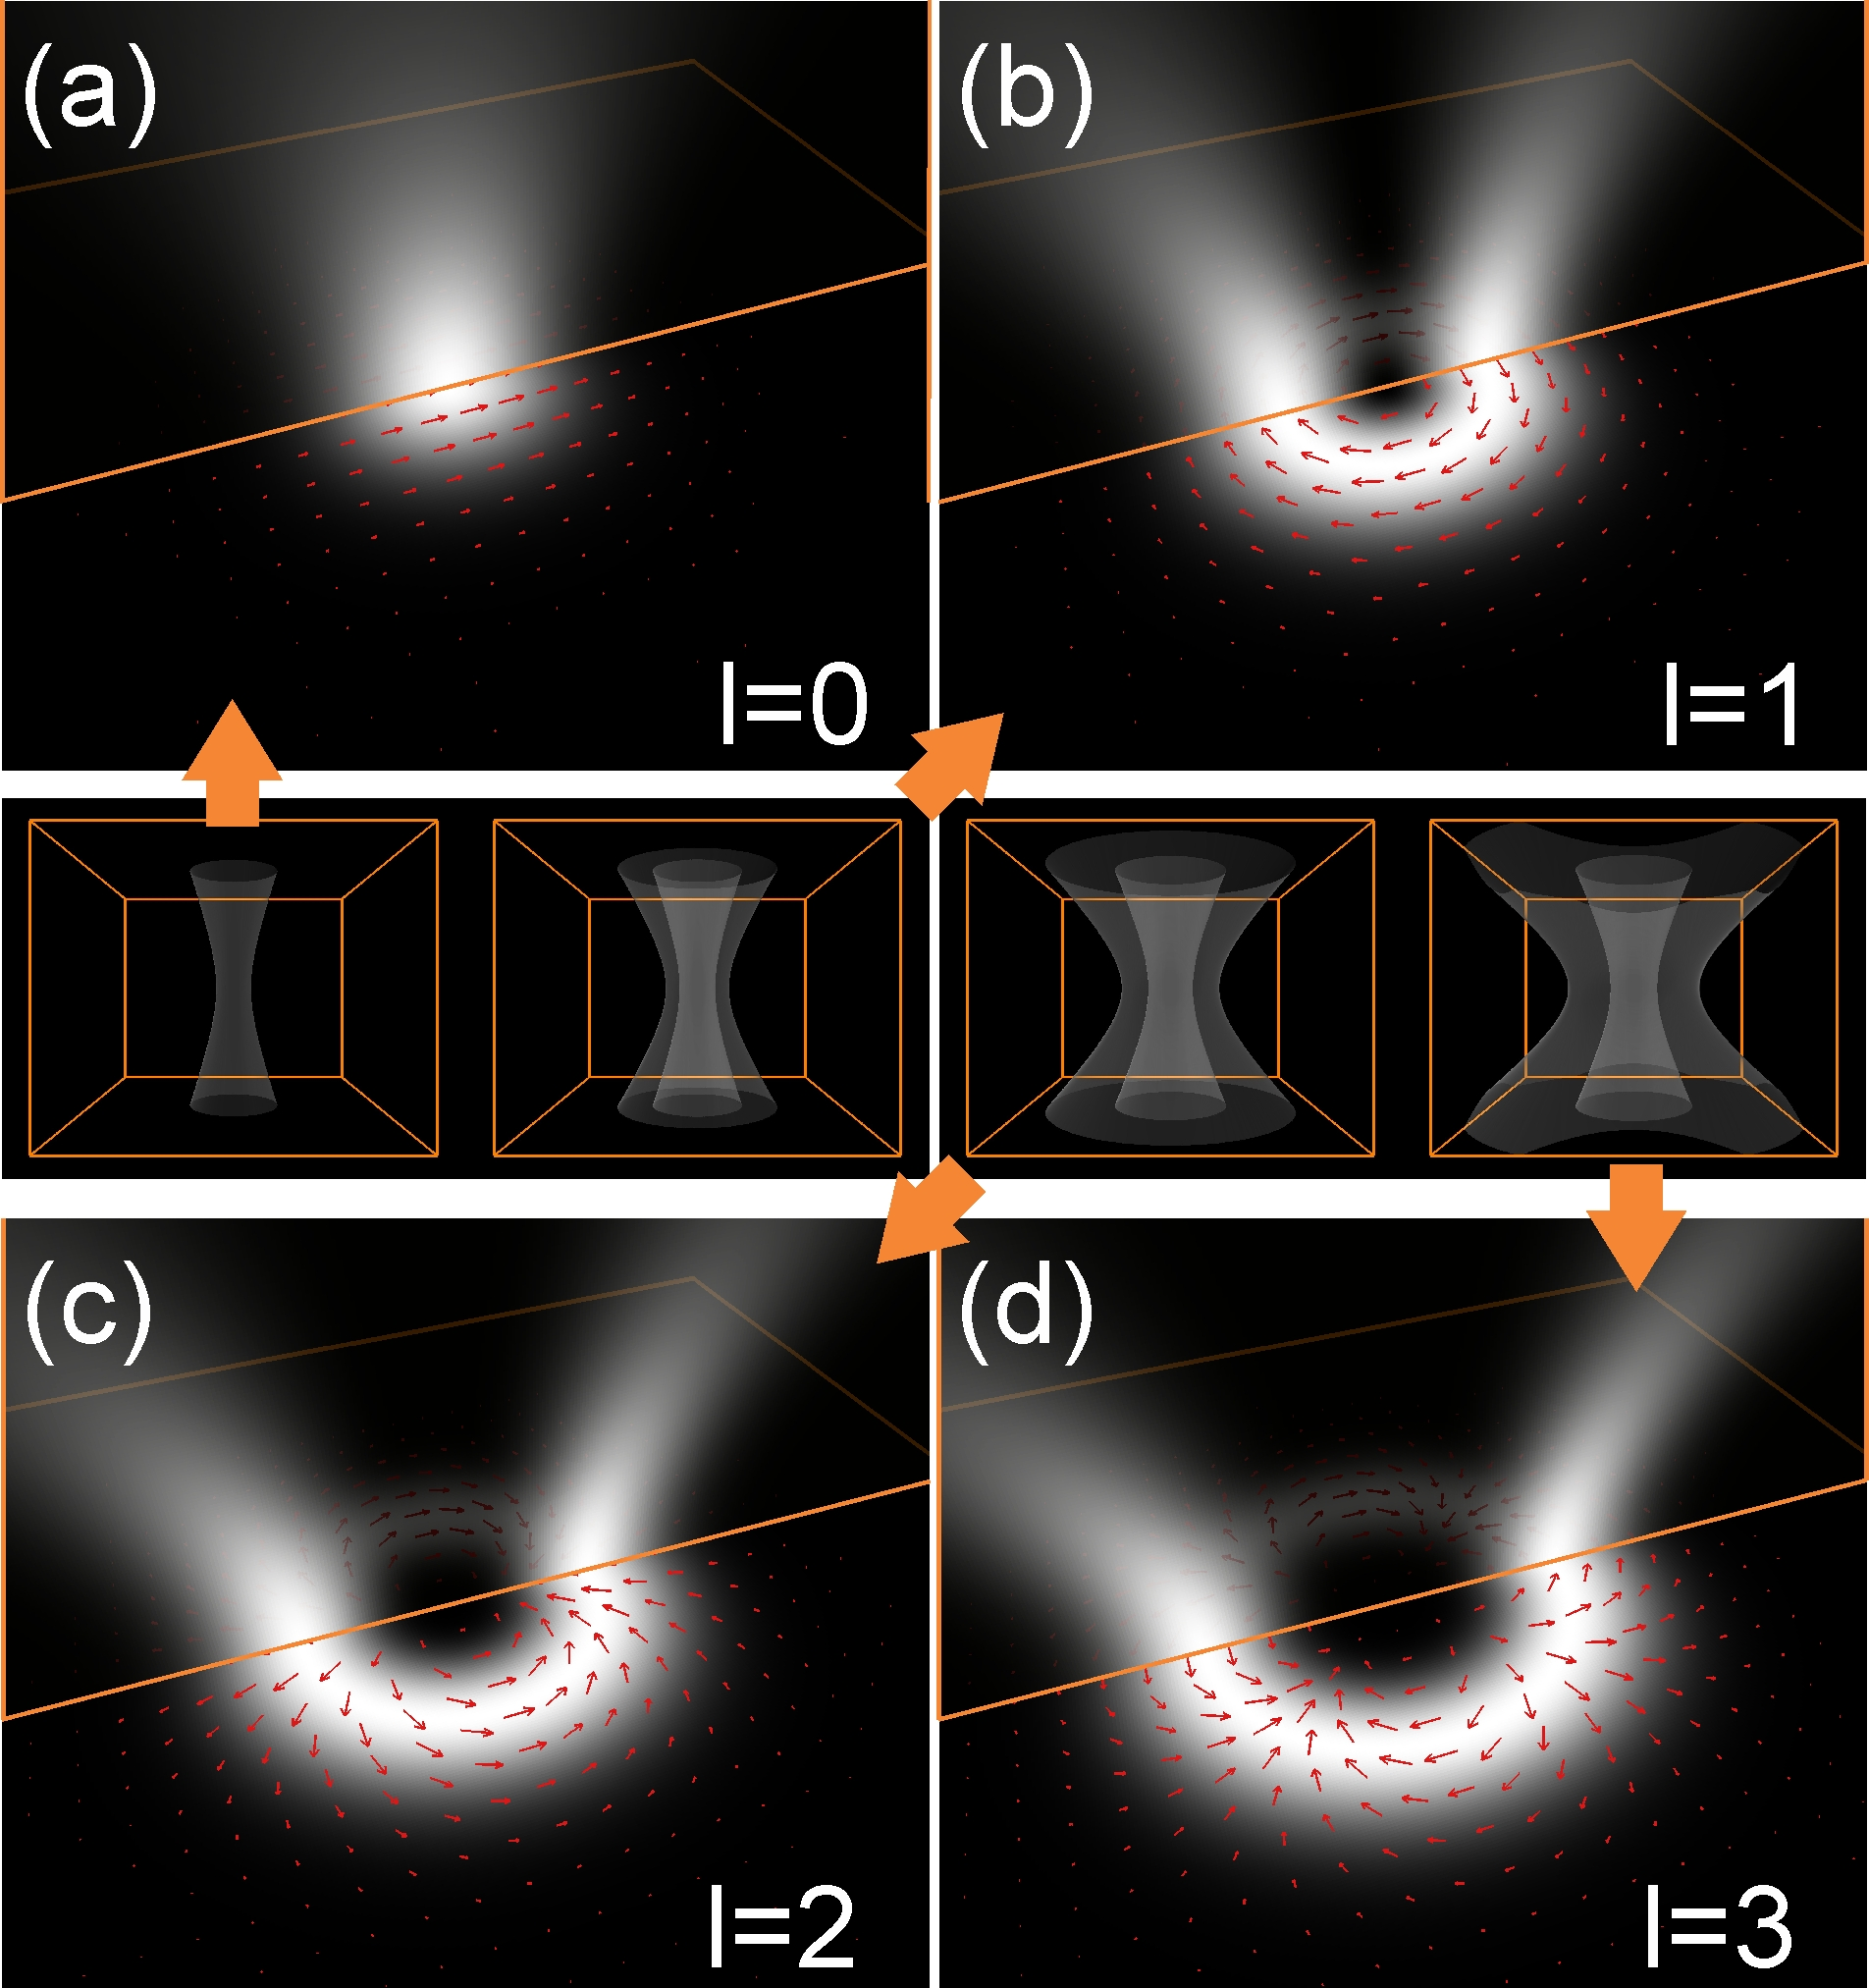
\includegraphics[width=.8\textwidth]{1_v6}
 \caption{Intenziteta in polarizacija v nekaterih Laguerre-Gaussovih na"cinih. Slike (a), (b), (c) in (d) prikazujejo snope z ovojnimi "stevili $l = 0,1,2,3$. Bela barva predstavlja obmo"cja z visoko intenziteto svetlobe v dveh ravninah, pravokotni in vzporedni s snopom. Rde"ce pu"s"cice prikazujejo polarizacijo svetlobe v ravnini grla snopa. \cite{porenta}}
 \label{fig:laguerre-gauss}
\end{figure}

Kljub topolo"ski podobnosti pa so defekti v polarizaciji svetlobe fizikalno zelo razli"cni od defektov v ureditvi teko"cega kristala. 
Deformacije elektromagnetnega polja ne nosijo elasti"cne energije, ki bi jo ravnovesno stanje minimiziralo. 
S primernimi opti"cnimi elementi lahko skonstruiramo svetlobo z defekti v polarizaciji, kot je npr. simetrijska ravnina z obratom polarizacije, ki bi v teko"cem kristalu razpadli zaradi previsoke energije. 

\section{Dielektri"cni tenzor v teko"cem kristalu}
\label{sec:dielektricnost}
Oblika in polarizabilnost molekul v teko"cem kristalu vplivata na njegove opti"cne lastnosti. 
Dielektri"cni tenzor v teko"cem kristalu je odvisen od molekularne anizotropije $\varepsilon_{a}^{\mathrm{mol}}$, direktorja in nematske stopnje reda $S$ in je neposredno povezan z nematskim tenzorjem ureditvenega paramtera $Q_{ij}$.
Dielektri"cni tenzor pogosto zapi"semo kot vsoto izotropnega in brezslednega dela \cite{degennes, ravnik-zumer-ldg}
\begin{align}
\label{eq:dielektricni-tenzor}
 \varepsilon_{ij} &= \overline\varepsilon \delta_{ij} + (\varepsilon_a)_{ij} = \overline\varepsilon\delta_{ij} + \frac{2}{3}\varepsilon_a^{\mathrm{mol}} Q_{ij}
\end{align}
Lastni vektorji tenzorja $Q_{ij}$ so direktor in dve pravokotni smeri, po zgornji zvezi pa so enake tudi lastne osi dielektri"cnega tenzorja. 
V enoosnem teko"cem kristalu je tako opti"cna os z izrednim lomnim koli"cnikom vzporedna z direktorjem. 

"Ce primerjamo ena"cbi (\ref{eq:dielektricna-sklopitev}) in (\ref{eq:dielektricni-tenzor}) opazimo dvosmerno povezavo med ureditvijo teko"cega kristala in elektromagnetnim poljem. 
Zaradi dielektri"cne sklopitve svetloba vpliva na ureditev teko"cega kristala, zaradi opti"cne anizotropije pa teko"ci kristal vpliva na "sirjenje svetlobe po njem. 
Ra"cunsko orodje, ki naj bi natan"cno napovedalo direktorsko polje ob prisotnosti svetlobe ali "sirjenje svetlobe skozi teko"ci kristal, bi moralo upo"stevati to dvosmerno povezavo in hkrati ra"cunati oboje. 
V praksi pa se pogosto zate"cemo k poenostavitvam oz. limitam mo"cnega ali "sibkega polja. 
"Ce je elektromagnetno polje dovolj mo"cno, se bo direktor orientiral v smeri polja, torej svetloba vedno "cuti izredni lomni koli"cnik. 
V tem re"zimu teko"ci kristal ne vpliva na "sirjenje svetlobe. 
"Ce pa je svetloba zelo "sibka, ne spremeni orientacije molekul in lahko privzamemo, da je direktorsko polje doloceno z drugimi mehanizmi, tipi"cno s povr"sinskim pogoji.. 
Mo"cno se razlikujeta tudi "casovni skali obeh pojavov, saj opti"cna polja pa nihajo s periodo okrog femtosekunde, metdem ko je tipi"cen relaksacijski "cas teko"cega kristala nekaj milisekund. 

V tem magistrskem delu sem se omejil le na "sirjenje svetlobe, pri "cemer je direktorsko polje dolo"ceno in "casovno nespremenljivo. 
Sama ra"cunska metoda pa je zasnovana tako, da je kompatibilna z obstoje"cimi programi za izra"cun ureditve teko"cih kristalov \cite{ravnik-zumer-ldg}. 
Z isto metodo bo v prihodnosti mogo"ce upo"stevati dvosmerno sklopitev med opti"cnim poljem in teko"cim kristalom, premostiti pa bo treba "se razliko v "casovnih skalah. 

\section{Povezava med defekti v teko"cem kristalu in defekti v opti"cnem polju}
Orientacijski red v teko"cem kristalu je tesno povezani z opti"cnimi polji. 
Med njimi obstaja dvosmerna povezava, opisana v poglavju \ref{sec:dielektricnost}. 
Podobno so med seboj povezani tudi defekti. 

Svetloba ob prehodu defekta v ureditvi teko"cega kristala lahko pridobi fazno singularnost, torej obmo"cje, kjer faza valovanja ni definirana. 
Primer je kro"zno polarizirana svetloba, ki preide skozi teko"cekristalno kapljico s to"ckastim defektom v sredini, kot je prikazano na sliki \ref{fig:defekt-kapljica}. 
V tem primeru svetloba dobi neni"celno vrtilno koli"cino $l$, na sredini pa nastane temna pika \cite{brasselet-droplet}. 

\begin{figure}[!htbp]
 \centering
 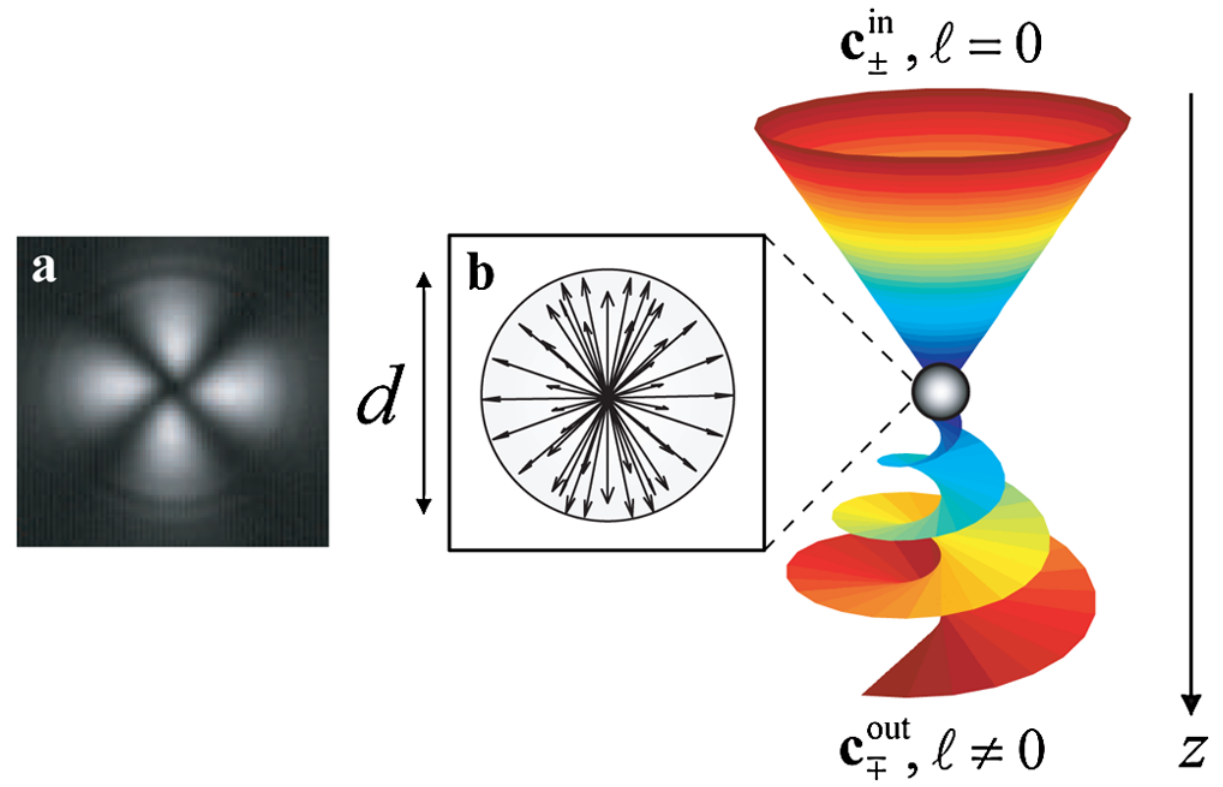
\includegraphics[width=.8\textwidth]{defekt-kapljica}
 \caption{Prehod kro"zno polarizirane svetlobe skozi kapljico z radialnim direktorskim profilom. Val z gladko valovno fronto ($l=0$) se deloma pretvori v stanje s singularnostjo v fazi ($l\neq 0$) \cite{brasselet-droplet}. Levo: (a) slika kapljice med prekri"zanima polarizatorja, ki potrjuje cilindri"cno simetri"cno direktorsko polje in (b) shema radialnega direktorja. }
 \label{fig:defekt-kapljica}
\end{figure}

S primerno ureditvijo teko"cega kristala lahko ustvarimo tudi svetlobo z ve"c singularnostmi. 
Z zunanjimi vplivi, na primer z elektri"cnim poljem, lahko teko"ci kristal preuredimo. 
Na ta na"cin lahko nastavljamo "stevilo in razporeditev defektov v svetlobnem polju \cite{brasselet-arrays}.
\begin{comment}
\begin{figure}[!htbp]
 \centering
 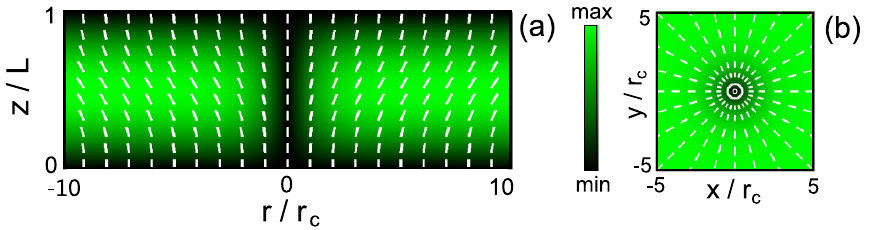
\includegraphics[width=.8\textwidth]{defekt-array-postavitev}
 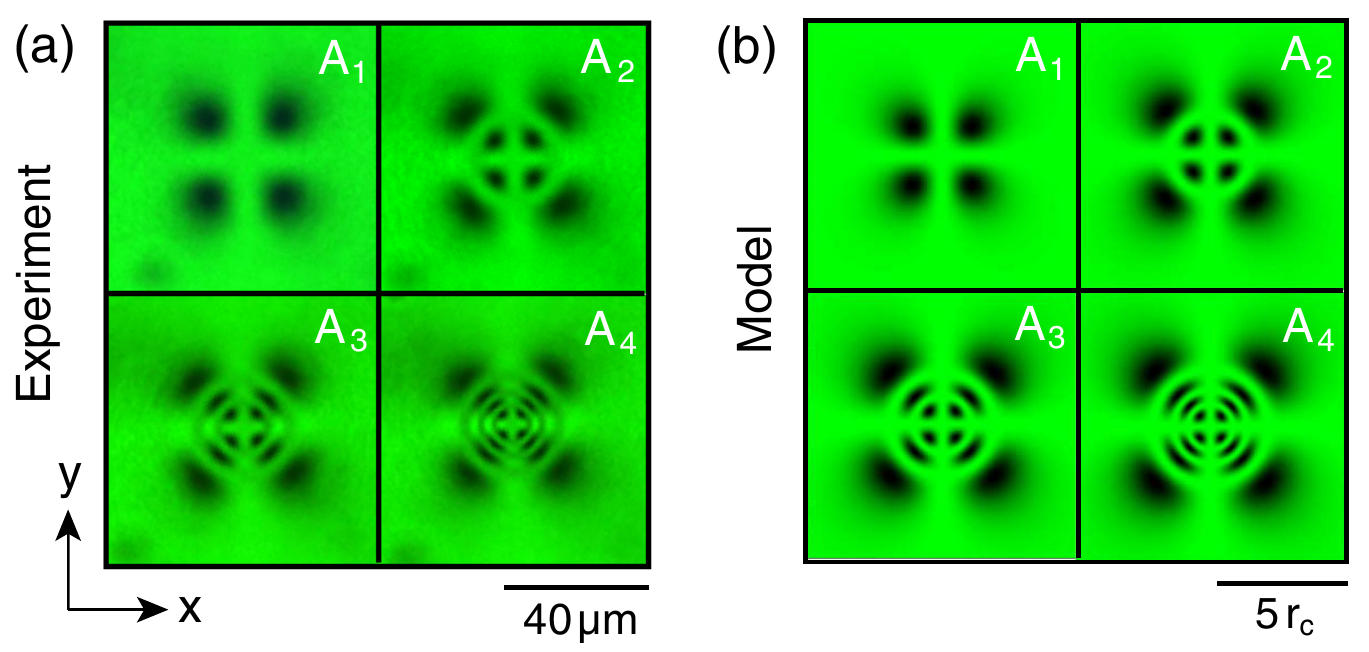
\includegraphics[width=.8\textwidth]{defekt-array-brasselet}
 \caption{Zgoraj: Pogled od strani in od zgoraj na ureditev teko"cega kristala. Direktorsko polje dodatno spreminjamo z elektri"cnim poljem. Spodaj: Eksperimentalna slika (levo) in rezultat numeri"cnega modela (desno) pri razli"cnih jakostih elektri"cnega polja. Vidnih je ve"c temnih pik na mestih s faznimi singularnostmi. \cite{brasselet-arrays}}
 \label{fig:defekt-arrays}
\end{figure}

\end{comment}

\begin{comment}
 
\subsection{Valj z dvojnim zvojem}

Holesteri"cni teko"ci kristal ima najni"zjo prosto energijo, "ce ima stalen zvoj. 
\todo{Mogo"ce kaj vec o double-twist cylindrih}

\begin{figure}
 \centering
 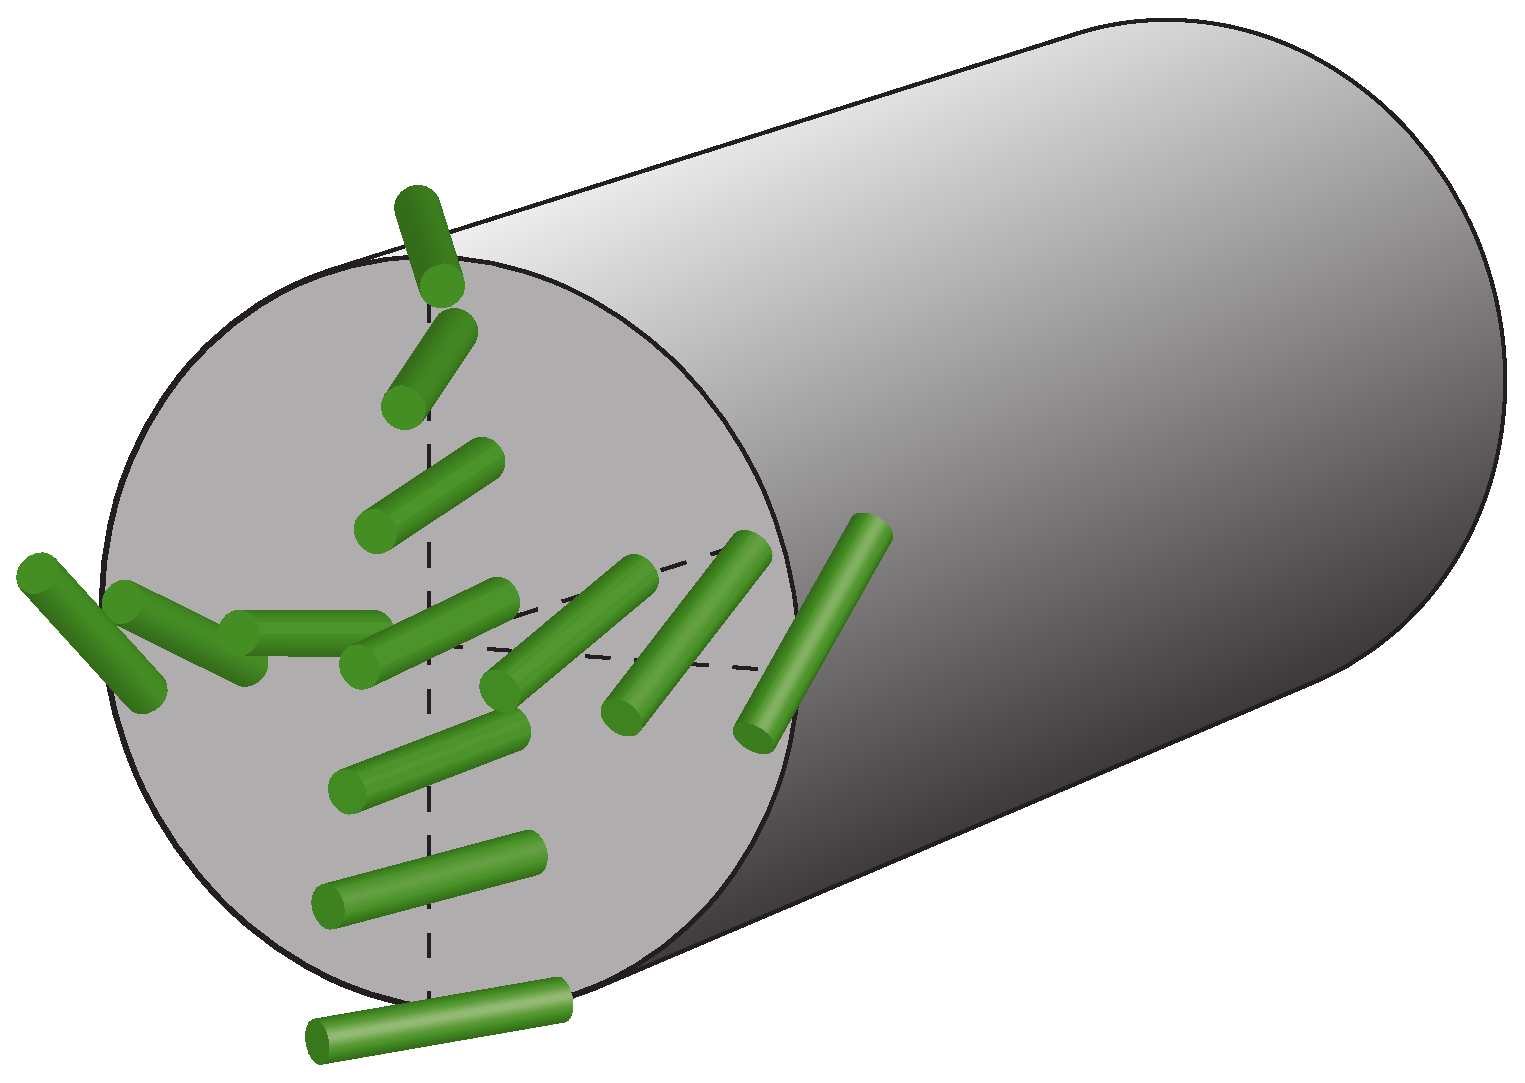
\includegraphics[width=.5\textwidth]{double-twist-cylinder-coles-morris}
 \caption{Shematski prikaz direktorja v valju z dvojnim zvojem. Na osi valja je direktor vzporeden z osjo, z oddaljenostjo od osi pa kot med osjo in direktorjem nara"s"ca linearno \cite{coles-morris}. }
 \label{fig:double-twist-cylinder}
\end{figure}

\end{comment}

\chapter{Numeri"cna metoda}

Za izracun propagacije svetlobe skozi mocno opticno aniztorpne tekocekristalne vzorce smo implementirali metodo kon"cnih diferenc v "casovni domeni \angl{\acf{FDTD}} \cite{taflove}. 
Pri tej metodi "casovno propagiramo elektri"cno in magnetno polje v vsaki to"cki po Maxwellovih ena"cbah. 

Pri numeri"cnem re"sevanju potrebujemo le tisti dve Maxwellovi ena"cbi, ki vsebujeta "casovne odvode polj. 
Konsistenca Maxwellovih ena"cb zagotavlja, da "ce prvi dve ena"cbi dr"zita na za"cetku, bosta avtomatsko izpolnjeni ob vsakem "casu\cite{taflove}. 
Izvore valovanja namesto z dodajanjem nabojev in tokov v vzorec raje simuliramo z robnimi pogoji, kot da valovanje prihaja od zunaj. 
Ta pristop je smiseln, saj v eksperimentih teko"ci kristal opazujemo tako, da svetimo skozenj. 

"Ce izrazimo "casovna odvoda in ena"cbi prepi"semo v brezdimenzijsko obliko ($c = \varepsilon_0 = \mu_0 = 1$), se glasita
\begin{align}
\label{eq:maxwell-base}
 \odvod{\vec{B}}{t} = -\nabla \times \vec{E}, \qquad \odvod{\vec{E}}{t} = \eps^{-1} (\nabla \times \vec{B} - \sigma \vec E)\,.
\end{align}

V zgornjih ena"cbah smo implicitno upo"stevali, da v celici ni prostih nabojev.
V ena"cbah nastopajo le prvi odvodi, ki jih za numeri"cno ra"cunanje nadomestimo s simetri"cnimi kon"cnimi diferencami
\begin{align}
 \frac{\partial y}{\partial x} \rightarrow \frac{y(x+\delta/2) - y(x-\delta/2)}{\delta}\,
\end{align}
kjer je $\delta$ korak diskretizacije, $y(x)$ pa poljubna skalarna funkcija. 
Na ta na"cin diskretiziramo krajevno in "casovno odvisnost vseh komponent elektromagnetnih polj. 

Znotraj teko"cega kristala lahko obi"cajno elektri"cno prevodnost zanemarimo in zato izpustimo "clen $\sigma \vec E$. 
Prevodnost pa je pomembna v robni plasti, kjer "zelimo absorpcijo valovanja. 

Zaradi simetrije Maxwellovih ena"cb bi na enak na"cin kot dielektri"cnost $\varepsilon$ lahko upo"stevali tudi magnetno permeabilnost $\mu$. 
Podobno bi lahko poleg elektri"cne prevodnosti $\sigma$ upo"stevali magnetne izgube $\sigma^\ast$. 

\section{Mre"za}

Pri diskretizaciji si lahko pomagamo z obliko obeh ena"cb. 
Za izra"cun "casovnega odvoda vsakega izmed polj $\vec{E}, \vec{B}$ potrebujemo le vrednosti drugega polja. 
Poleg tega obe ena"cbi povezujeta "casovni odvod enega polja s krajevnim odvodom drugega. 
Zaradi obeh opisanih lastnosti lahko dvignemo red metode, in s tem izbolj"samo natan"cnost, "ce vrednosti polj poznamo ob razli"cnih "casih in na razli"cnih mestih \cite{taflove}. 

Obi"cajne implementacije metode \acs{FDTD} gredo "se korak dlje, tako da so tudi posamezne komponente elektri"cnega in magnetnega polja definirane na razli"cih to"ckah \cite{yee, yee-lattice}.
Tak"sno mre"zo je predlagal Yee in izkori"s"ca dejstvo, da pri "casovnem odvodu vsake komponente posameznega polja nastopata le krajevna odvoda ostalih dveh komponent drugega polja. 
Z ustrezno izbiro to"ck, kjer so definirane posamezne komponente, vse krajevni odvode potrebujemo ravno na sredini med ustreznima to"ckama mre"ze. 
Za u"cinkovito delovanje pa tak"sna mre"za zahteva, da je dielektri"cni tenzor $\eps$ diagonalen, njegove komponente pa morajo biti znane na razli"cnih to"ckah mre"ze. 
V praznem prostoru ali v trdnih kristalih temu pogoju lahko zadostimo, po mo"znosti z vrtenjem koordinatnega sistema.

V teko"cih kristalih je dielektri"cni tenzor anizotropen in se mo"cno spreminja s krajem. 
Zaradi krajevnega spreminjanja ne moremo tako obrniti koordinatnega sistema, da bi bil tenzor diagonalen v vseh to"ckah. 
Poleg tega obstoje"ci programi za modeliranje ureditve teko"cih kristalov podajo vse komponente dielektri"cnega tenzorja na istem mestu \cite{ravnik-zumer-ldg}.
Ta omejitev mo"cno zmanj"sa prednosti Yeejeve mre"ze, zato smo raje uporabili svojo. 
Odlo"cili smo se za srednjo pot, kjer sta polji $\E$ in $\B$ definirani ob razli"cnih "casih in na razli"cnih to"ckah mre"ze, vse tri komponente vsakega izmed polj pa so podane na istem mestu. 
Obe mre"zi prikazuje slika \ref{fig:lattice}. 

\begin{figure}[h]
\centering
 \subfigure{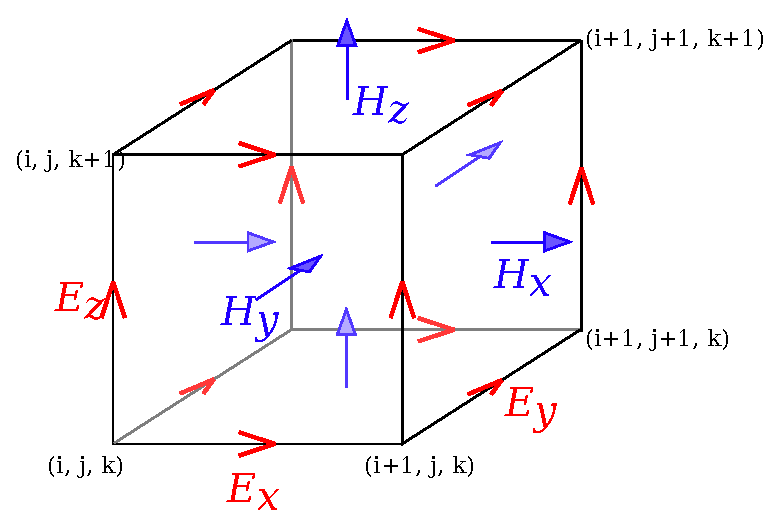
\includegraphics[width=.5\textwidth]{Yee-cube}}
 \subfigure{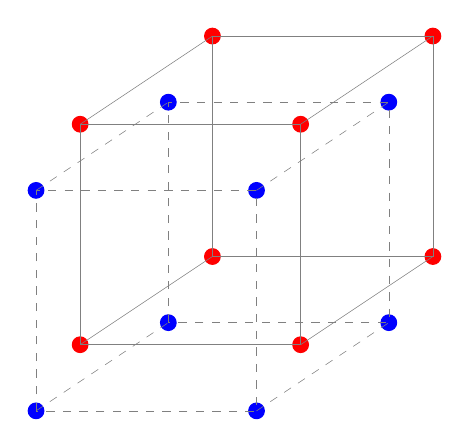
\begin{tikzpicture}[scale=1.4]
    
    \foreach \x in {0,1}{
      \foreach \y in {0,1}{
        \node[mpoint] at (2*\x,2*\y) {}; 
        \node[mpoint] at (2*\x+1.2,2*\y+0.8) {}; 
        \node[epoint] at (2*\x+1.6,2*\y+1.4) {};
        \node[epoint] at (2*\x+1.6-1.2,2*\y+1.4-0.8) {};
        \draw[mgrid] (2*\x,2*\y) -- (2*\x+1.2,2*\y+0.8);
        \draw[egrid] (2*\x+1.6,2*\y+1.4) -- (2*\x+1.6-1.2,2*\y+1.4-0.8);
      }
    }
    
    \draw[mgrid] (0,0) rectangle (2,2);
    \draw[mgrid] (1.2,0.8) rectangle (3.2,2.8);
    \draw[egrid] (1.6,1.4) rectangle (3.6,3.4);
    \draw[egrid] (1.6-1.2,1.4-0.8) rectangle (3.6-1.2,3.4-0.8);

            \end{tikzpicture}}
\caption{Levo: Yeejeva celica, pri kateri so komponente elektri"cnega polja znane na razpolovi"s"cih robov konce, komponente magnetnega polja pa v sredi"s"cih ploskev \cite{yee-lattice}. Desno: Celica, ki smo jo uporabili pri izra"cunih. Komponente elektri"cnega polja so znane v ogli"s"cih kocke, komponente magnetnega polja pa v njenem sredi"s"cu. V obeh primerih sta elektri"cno in magnetno polje dolo"cena ob razli"cnih "casih, kar na sliki ni prikazano.}
\label{fig:lattice}
\end{figure}

Za ra"cun potrebujemo "se inverz dielektri"cnega tenzorja, ki pa se med propagacijo svetlobe ne spreminja, zato ga lahko izra"cunamo predhodno. 
Lahko neposredno predpi"semo vse komponente tenzorja, bolj priro"cno pa je podati le direktor in stopnjo reda, iz katerih nato izra"cunamo dielektri"cni tenzor in njegov inverz. 
Pomembno je le, da je znan na istem mestu kot $\E$ (rde"ce to"cke na sliki \ref{fig:lattice}).

\section{Postopek re"sevanja}
Na izbrani mre"zi ne moremo neposredno izra"cunati rotorja polj, ker ta ni definiran v pravih to"ckah. 
Elektri"cno polje je definirano na ogli"s"cih kocke, zato so krajevni odvodi tega polja definirani na razpolovi"s"cih robov, potrebujemo pa jih na mestu magnetnega polja, torej v sredi"s"cu kocke. 
V svoji metodi sem za odvod polja po vsaki koordinati v sredi"s"cu kocke uporabil povpre"cje odvodov na vseh "stirih robovih, ki potekajo v smeri izbrane koordinate, kot prikazuje slika \ref{fig:lattice-derivatives}. 

\begin{figure}[h]
\centering
 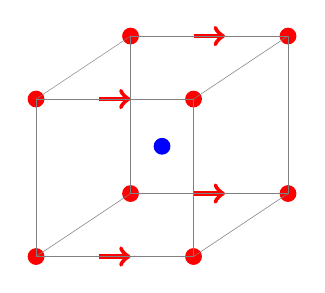
\begin{tikzpicture}
  \foreach \y in {0,1}{
      \foreach \x in {0,1}{
        \node[epoint] at (2*\x+1.6,2*\y+1.4) {};
        \node[epoint] at (2*\x+1.6-1.2,2*\y+1.4-0.8) {};
        \draw[egrid] (2*\x+1.6,2*\y+1.4) -- (2*\x+1.6-1.2,2*\y+1.4-0.8);
      }
      \draw[->,red,ultra thick] (1.4+1,2*\y+1.4) -- +(0.4,0);
      \draw[->,red,ultra thick] (0.2+1,2*\y+0.6) -- +(0.4,0);
    }
    
    \draw[egrid] (1.6,1.4) rectangle (3.6,3.4);
    \draw[egrid] (1.6-1.2,1.4-0.8) rectangle (3.6-1.2,3.4-0.8);
    
    \node[mpoint] at (2,2) {};
 \end{tikzpicture}
 \caption{
 Krajevni odvodi komponent polja $\E$ v smeri $x$ so definirani na "stirih robovih, ozna"cenih s pu"s"cicami. 
 Vrednost potrebujemo v sredi"s"cu kocke (modra pika), zato sem uporabil povpre"cje "stirih vrednosti na robu. 
 }
 \label{fig:lattice-derivatives}
\end{figure}

V primerjavi z Yeejevo celico povpre"cenje pove"ca "cas ra"cunanja, saj moramo namesto vsakega krajevnega odvoda izra"cunati "stiri. 
Na sre"co pa si vsak rob delijo "stiri kocke, tako da se s sprotnim shranjevanjem odvodov lahko izognemo ve"ckratnemu ra"cunanju istega odvoda. 
Na ta na"cin je "stevilo ra"cunskih operacij blizu tistemu, ki bi ga potrebovali z uporabo Yeejeve mre"ze. Na izbrani mre"zi so vse komponente elektri"cnega polja znane ob "casih $k\Delta t$, $k\in\mathbf{N}$, in sicer na polo"zajih, kjer so vse tri prostorske koordinate celo"stevilski ve"ckratniki enote diskretizacije $\Delta x$. 
Magnetno polje je znano ob "casih $(k+1/2)\Delta t$ na polo"zajih, kjer so vse tri prostorske koordinate polcelo"stevilski ve"ckratniki $\Delta x$. 
V kompoktnem zapisu ozna"cimo
\begin{align}
 E_\alpha|_{i,j,k}^n &= E_\alpha\Big(i\Delta x, j\Delta y, k\Delta z, n \Delta t\Big) \\
 H_\alpha|_{i,j,k}^n &= H_\alpha\left(\left(i+1/2\right)\Delta x, \left(j+1/2\right)\Delta y, \left(k+1/2\right)\Delta z, \left(n+1/2\right) \Delta t\right)
\end{align}
in zapi"semo krajevne odvode vsake komponente elektromagnetnih polj
\newcommand{\sumij}[2]{\substack{ #1' = #1,\, #1+1 \\ #2' = #2,\, #2+1}}
\begin{align}
 \label{eq:diskretni-odvodi}
 \left.\frac{\partial \phi}{\partial x}\right|_{i,j,k}^n &= \frac{1}{4\Delta x}\sum_{\sumij{k}{j}} \phi|_{i+1,j',k'}^{n} - \phi|_{i,j',k'}^{n} \\
 \left.\frac{\partial \phi}{\partial y}\right|_{i,j,k}^n &= \frac{1}{4\Delta y}\sum_{\sumij{i}{k}} \phi|_{i',j+1,k'}^{n} - \phi|_{i',j,k'}^{n} \\
 \left.\frac{\partial \phi}{\partial z}\right|_{i,j,k}^n &= \frac{1}{4\Delta z}\sum_{\sumij{j}{i}} \phi|_{i',j',k+1}^{n} - \phi|_{i',j',k}^{n}	
\end{align}
kjer je $\phi$ poljubna komponenta elektri"cnega ali magnetnega polja.
Rotorje polj, ki nastopajo v Maxwellovih ena"cbah, izrazimo z odvodi
\begin{align}
 \label{eq:diskretni-rotor}
 (\nabla\times\vec A)_x|_{i,j,k}^n &= \left.\frac{\partial A_z}{\partial y}\right|_{i,j,k}^n - \left.\frac{\partial A_y}{\partial z}\right|_{i,j,k}^n\\
 (\nabla\times\vec A)_y|_{i,j,k}^n &= \left.\frac{\partial A_x}{\partial z}\right|_{i,j,k}^n - \left.\frac{\partial A_z}{\partial x}\right|_{i,j,k}^n\\
 (\nabla\times\vec A)_z|_{i,j,k}^n &= \left.\frac{\partial A_y}{\partial x}\right|_{i,j,k}^n - \left.\frac{\partial A_x}{\partial y}\right|_{i,j,k}^n
\end{align}
kjer je $\vec A$ elektri"cno ali magnetno polje. 

Pri zgornjem zapisu je rotor polja definiran med to"ckami mre"ze, torej na mestih $A_\alpha|_{i+1/2,j+1/2,k+1/2}$. 
Ker rotor polja potrebujemo pri "casovnem odvodu drugega opti"cnega polja, ki je definiran ravno na teh mestih, je zgornji zapis primeren za izbrano mre"zo. 
V splo"snem je diskretizacija lahko anizotropna, v vseh nadaljnjih izra"cunih pa smo uporabili kvadratno mre"zo, kjer je $\Delta x = \Delta y = \Delta z$. 
Maxwellove ena"cbe v tem zapisu se glasijo
\begin{align}
 E_\alpha|_{i,j,k}^{n+1} &= E_\alpha|_{i,j,k}^n + \Delta t \times (\varepsilon^{-1})_{\alpha\beta}|_{i,j,k} \times (\nabla\times \vec H)_\beta|_{i-1,j-1,k-1}^{n} \label{eq:disk-E}\\
 H_\alpha|_{i,j,k}^{n+1} &= H_\alpha|_{i,j,k}^n + \Delta t \times (\nabla\times \vec E)_\beta|_{i,j,k}^{n+1} \label{eq:disk-H}
\end{align}
Iz zgornjih dveh ena"cb je razvidno, da lahko obe polji ra"cunamo izmeni"cno. 
"Ce poznamo elektri"cno polje ob "casu $n\Delta t$ in magnetno polje ob "casu $(n+1/2)\Delta t$, lahko po ena"cbi izra"cunamo (\ref{eq:disk-E}) izra"cunamo elektri"cno polje ob "casu $(n+1)\Delta t$, nato pa po ena"cbi (\ref{eq:disk-H}) "se magnetno polje ob "casu $(n+3/2)\Delta t$. Izmeni"cno ra"cunanje lahko ponavljamo poljubno dolgo. 

Pomembna lastnost obeh zgornjih ena"cb je, da med ra"cunanje enega izmed polj potrebujemo le vrednosti drugega polja, ne pa tudi istega polja na sosednjih mestih. 
"Casovni odvodi istega polja na razli"cnih mestih so med seboj popolnoma neodvisni. 
Vsak korak metode, torej ra"cunanje enega izmed polj, lahko razdelimo na veliko "stevilo neodvisnih ra"cunskih enot. 
To omogo"ca paralelno izvajanje programa na ra"cunalnikih z ve"c jedri, kot so ra"cunalni"ske gru"ce, pa tudi novej"si osebni ra"cunalniki. 

Pri zgornjem zapisu smo implicitno privzeli, da je dielektri"cne tenzor $\varepsilon_{\alpha\beta}$ odvisen od kraja, ne pa od "casa. 
Privzetek je smiseln v trdnih snoveh, pa tudi v teko"cih kristalih, saj je zna"cilen relaksacijski "cas snovi mnogo ve"cji od periode nihanja opti"cnih polj. 
Ker nastopa pri "casovnem odvodu elektri"cnega polja, mora biti podan na istih mestih kot $E_\alpha$, torej v to"ckah s celo"stevilskimi koordinatami. 

\section{Izvor valovanja}

V ena"cbah (\ref{eq:maxwell-base}) ne nastopajo izvori valovanja, zato jih moramo modelirati z robnimi pogoji. 
To je v skladu z eksperimenti, saj svetloba pride od zunaj, zanima pa nas predvsem njeno "sirjenje skozi snov. 

Poljubno vpadno valovanje lahko modeliramo z robnimi pogoji, "ce izkoristimo linearnost Maxwellovih ena"cb. 
Elektri"cno in magnetno polje lahko namre"c razcepimo na vsoto vpadnega in sipanega valovanja \cite{taflove}. 
Tak"sen razcep polja je mo"zen le, "ce je "sirjenje vpadnega valovanja dobro znano. 
To velja za ravne valove, pa tudi za bolj zapletene primere kot so Laguerre-Gaussovi snopi. 
Mre"zo zato razdelimo na dve obmo"cji, v notranjem obmo"cju ra"cunamo s skupnim poljem, v zunanjem pa polje razcepimo in shranjujemo le sipani del.
Opti"cno anizotropna snov mora biti v celoti v notranjem obmo"cju, izvor valovanja modeliramo na prehodu med obmo"cjema. 

\begin{figure}[h]
 \centering
 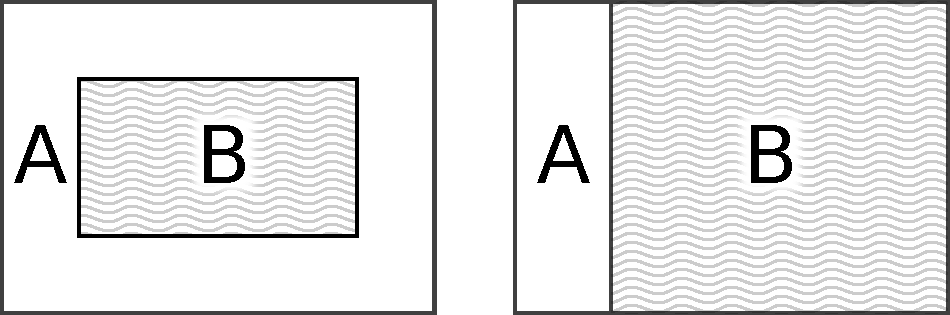
\includegraphics[width=.8\textwidth]{wave-source-regions}
 \caption{Delitev mre"ze na dve obmo"cji. V obmo"cju \textbf{A} ra"cunamo le z sipanim valovanjem, v obmo"cju \textbf{B} pa s celotnim valovanjem. Delitev na levi sliki je primerna, "ce je razlika med lomnima koli"cnikoma \textbf{A} in \textbf{B} dovolj majhna. V nasprotnem primeru uporabimo delitev na desni sliki. }
 \label{fig:wave-source-regions}
\end{figure}

Delitev na notranje in zunanje obmo"cje je u"cinkovita, "ce se efektivni lomni koli"cnik v notranem obmo"cju ne razlikuje mo"cno od zunanjega. 
V tem primeru je fazna razlika na zadnji stranici notrenjega obmo"cja dovolj majhna, da pretvorba na sipano valovanje odstrani ve"cino valovanja. 
"Ce pa je fazna razlika primerljiva s $\pi/2$ ali ve"cja, lahko odstranitev vpadnega vala celo pove"ca amplitudo valovanja. 
To se zgodi npr. v teko"cekristalnem valovodu, ki je mnogo dalj"si od valovne dol"zine svetlobe. 
Takrat je bolj u"cinkovito upo"stevati izvor valovanja le na vpadni strani, na drugi strani pa postavimo plast, ki absorbira valovanje. 

Delitev na zunanje in notranje obmo"cji, ki je prikazana na levi strani slike \ref{fig:wave-source-regions}, smo uporabili le s preprostimi primeri za preverjanje delovanja metode. 
Vse ostale izra"cune smo izvedli z delitvijo na desni strani. 
Na sliki je velikost obmo"cja \textbf{A} pretirana zaradi preglednosti. 
V vseh primerih je bila debelina obmo"cja \textbf{A} enaka dva koraka mre"ze. 

\section{Robni pogoji}

"Ce imamo na robu celice dolo"ceno vrednost elektri"cnega in magnetnega polja, se bo celotno valovanje odbilo in vrnilo v celico. 
"Ce so dolo"ceni odvodi polj, ali pa linearna kombinacija vrednosti in odvodov, se bo valovanje odbilo z dolo"cenim faznim zamikom. 
Tega si ne "zelimo, saj pri izvedbi ekperimentov obi"cajno svetloba najprej preide skozi vzorec, nato pa jo zajamemo in preu"cimo. 
Odbita svetloba, ki bi se vrnila v vzorec, bi zmotila svetlobno polje in ote"zila opazovanje. 
Za modeliranje tak"snega eksperimenta bi morali uporabiti zelo veliko prazno obmo"cje, v katerega bi se svetloba "sirila, kar pa mo"cno upo"casni delovanje metode. 
"Sirjenje v prazen prostor brez odboja pa lahko u"cinkoviteje simuliramo z uporabo absorbirajo"cega robnega pogoja \angl{\ac{ABC}}. 
Obstaja ve"c razli"cnih implementacij absorbirajo"cih robnih pogojev, v zadnjem "casu se najve"c uporablja t.i. popolnoma ujemajo"ca plast \angl{\ac{PML}} \cite{taflove,berenger}. 

Material v plasti \acs{PML} zagotavlja eksponentno pojemanje vpadnega vala, neodvisno od njegove frekvence in smeri "sirjenja. 
Absorpcijo valovanja dose"zemo z uporabo elektri"cne prevodnosti $\sigma$ in magnetnih izgub $\sigma^\ast$. 
Odboju na meji med notranjostjo celice in plastjo \acs{PML} se izognemo, "ce izgube v robni plasti zado"s"cajo pogoju $\sigma/\sigma^\ast = \eps_1/\mu_1$, kjer sta $\eps_1$ in $\mu_1$ dielektri"cnost in magnetna permeabilnost v notranjosti. 
To ujemanje izgub odpravi odboj na meji le za valovanje, ki vpada pravokotno na mejo. 
Odboj valovanja pod poljubnim kotom prepre"cimo, "ce vsako komponento elektri"cnega in magnetnega polja razdelimo na dva prispevka. 
Tak material je nefizikalen, saj imamo dodatne prostostne stopnje, polje pa ne sledi ve"c Maxwellovim ena"cbam. 

Komponenta $E_x$ elektri"cnega polja vala v obi"cajnem izotropnem mediju z dielektri"cnostjo $\eps$ in elektri"cno prevodnostjo $\sigma$ zado"s"ca Maxwellovi ena"cbi
\begin{align}
 \eps \odvod{E_x}{t} + \sigma E_x = \odvod{H_z}{y} - \odvod{H_y}{z}\;.
\end{align}
V plasti \acs{PML} pa elektri"cno polje razdelimo na dva prispevka, $E_x = E_{xy} + E_{xz}$, ki zado"s"cata ena"cbam
\begin{align}
 \eps \odvod{E_{xy}}{t} + \sigma_y E_{xy} &= \odvod{H_z}{y} = \odvod{}{y}(H_{zx} + H_{zy}) \\
 \eps \odvod{E_{xz}}{t} + \sigma_z E_{xz} &= -\odvod{H_y}{z} = -\odvod{}{z}(H_{yx} + H_{yz});,
\end{align}
kjer smo razcepljenima komponentoma pripisali razli"cni prevodnosti. 
Na enak na"cin so razcepljene ostale komponente eletri"cnega in magnetnega polja. 

Razcep polj omogo"ca anizotropno absorpcijo v robni plasti. 
Izberemo lahko tak"sne vrednosti za $\sigma_i$ in $\sigma^\ast_i$, da se absorbira le komponenta, ki se "siri pravokotno na plast. 
Komponenta svetlobe, ki se "siri vzporedno s plastjo, se ohrani in potuje znotraj robne plasti, tako da ne zmoti valovanja v celici. 
Na ta na"cin prepre"cimo odboj valovanja na meji med notranjostjo in plastjo \acs{PML} pri poljubnem vpadnem kotu valovanja. 
Primer postavitve plasti \acs{PML}, ki zadosti temu pogoju, je na sliki \ref{fig:pml-shema}. 

\begin{figure}[!htbp]
 \centering
 \def\svgwidth{.4\textwidth}
 \input{./Slike/pml.pdf_tex}
 \caption{Shema postavitve plasti \acs{PML} okrog ombo"cja, v katerem opazujemo propagacjo svetlobe. V rumenih obmo"cjih je neni"celna prevodnost $\sigma_x$, v modrih je neni"celna le $\sigma_y$, v zelenih obmo"cjih pa sta prisotni obe. Tak"sna postavitev prepre"cuje odboj svetlobe pri poljubnem vpadnem kotu \cite{taflove}. }
 \label{fig:pml-shema}
\end{figure}

\section{Absorpcija na robu}
Za prepre"cevanje odboja na stranskih ploskvah smo uporabili absorbirajo"ce robne pogoje. 
Plast \acs{PML} nam omogo"ca, da imamo material s poljubno velikimi izgubami, pa vseeno ne dobimo odboja na meji, vse dokler so elektri"cne in magnetne izgube v primernem razmerju. 
V praksi pa se zaradi diskretizacije vseeno nekaj valovanja odbije na meji med notranjostjo celice in robno plastjo. 
Najti moramo torej ravnote"zje med dvema prispevkoma: "ce so izgube majhne, bo del valovanja pri"sel skozi robno plast in se odbil na zunanjem robu. 
"Ce pa so izgube prevelike, se bo del valovanja odbil "ze na notranjem robu. 
Oba prispevka lahko zmanj"samo, "ce pove"camo debelino robne plasti, ampak s tem se pove"ca tudi "cas ra"cunanja. 
Odboj na notranji steni pa lahko omilimo, "ce se izognemo ostri meji in izgube zvezno nara"s"cajo od notranjosti proti robu. 
V literaturi \cite{taflove} priporo"cajo poten"cno nara"s"canje izgub, $\sigma \propto (d-d_0)^{p}$, kjer je $d$ oddaljenost od zunanjega roba, $d_0$ pa debelina plasti. 

Za nekaj vrednosti $p$ smo izra"cunali odbojnost robne plasti z debelino 10 enot diskretizacije. 
Rezultati so prikazani na sliki \ref{fig:test-absorption}. 

\begin{figure}[!htbp]
 \input{g_test_absorption}
 \caption{Odbojnost robne plasti v odvisnosti od povpre"cne prevodnosti $\overline{\sigma}$ pri razli"cnih profilih elektri"cnih in magnetnih izgub. Najbolje se izka"ze material, kjer izgube nara"s"cajo kvadratno z oddaljenostjo od roba celice ($p=2$). Debelina robnega sloja je 16 enot diskretizacije, valovna dol"zina svetlobe pa 10 enot. Pri tej debelini dose"zemo, da je intenziteta odbitega "zarka pet velikostnih redov ni"zja od intenzitete vpadnega "zarka. }
 \label{fig:test-absorption}
\end{figure}

V primeru, da v plasti ni izgub, je njena odbojnost enaka 1, saj gre celotno valovanje skozi plast in se odbije na zunanji meji. 
"Ce izgube malo pove"camo, odbojnost v vseh primerih strmo pade. 
Pri profilih, kjer imamo nezveznost v izgubah ali v njihovem odvodu ($p<2$) pa odbojnost kmalu za"cne spet nara"s"cati, saj postane odboj na notranji meji "ze opazen.
Pri ve"cjih potencah lahko izgube "se pove"camo in s tem dose"zemo ni"zjo odbojnost plasti. 
V zgornjem primeru se za najbolj"si profil izka"ze kvadratno nara"s"canje absorpcije, zato smo za vse nadaljnje ra"cune uporabili tak"sno plast. 
Z debelino robne plasti 16 enot in s primerno izbiro za prevodnost $\sigma$ v robnem pasu lahko dose"zemo, da je odbito valovanje za 5 velikostnih redov "sibkej"se od vpadnega. 
Pri uporabljeni lo"cljivosti metode je debelina plasti med eno in dvema valovnima dol"zinama svetlobe. 



\chapter{Primeri uporabe metode}

\section{Izotropen dielektrik}
Prvi preizkus metode, ki smo ga opravili, je "sirjenje svetlobe skozi izotropen dielektrik, kot je npr. prazen prostor. 
Prazen prostor je modeliran kot snov, kjer je dielektri"cni tenzor uniformen in izotropen. 
"Ce na eno stran celice postavimo planarni izvir ravnega valovanja, pri"cakujemo ravne valove po celotnem mediju. 

Pri tem preizkusu sta lomna koli"cnika v obeh obmo"cjih enaka, zato smo mre"zo razdelili na notranje in zunanje obmo"cje, izvor valovanja pa smo postavili po celotnem robu med obmo"cjema. 
Prikaz valovanja na sliki \ref{fig:test-plane} potrjuje pravilnost metode, saj res vidimo ravne valove s konstantno frekvenco in valovno dol"zino. 

\begin{figure}[h]
 \centering
 \begin{overpic}[width=.45\textwidth]{g_test_plane}
  \put(20,66){\color{white} \large \bf Valovanje \Huge $\rightarrow$}
  \put(10,2){\color{white} \large \bf $\mathbf{z \rightarrow}$}
  \put(2,17){\color{white} \large \bf $\mathbf{\uparrow}$}
  \put(2,10){\color{white} \large \bf $\mathbf{y}$}
  \put(0,37){\color{black} \hdashrule{0.46\textwidth}{1pt}{4pt 2pt}}
 \end{overpic}
 \hspace{-2mm}
 \begin{picture}(10,75)
 \thicklines
  \put(0,74){\line(1,6){12}}
  \put(0,74){\line(1,-6){12}}
 \end{picture}
 \hspace{-2mm}
 \begin{overpic}[width=.45\textwidth]{g_test_plane_profile}
  \put(2,10){\color{white} \large \bf $\mathbf{z}$}
  \put(0,6){\color{white} \large \bf $\mathbf{\rightarrow}$}
  \put(2,37){\color{white} \large \bf $\mathbf{\uparrow}$}
  \put(2,30){\color{white} \large \bf $\mathbf{t}$}
 \end{overpic}
\caption{Levo: Trenutna slika valovanja v celici. Vidni so ravni valovi, rumena barva prikazujejo obmo"cja s pozitivno komponento $E_x$, modra z negativno, rde"ca pa obmo"cja brez elektri"cnega polja. Desno: Presek po "crtkani "crt	i ob razli"cnih "casih. Navpi"cna os predstavlja "cas; valovi potujejo v desno s konstantno hitrostjo, na levi je izvor valovanja, na desni pa ponor. }
\label{fig:test-plane}
\end{figure}

Na obeh slikah opazimo notranjost celice z valovanjem in rob, kjer valovanja ni.
To je posledica modeliranja izvora valovanja okrog in okrog celice, kot je prikazano na levi strani slike \ref{fig:wave-source-regions}.
Valovanje se "siri od leve proti desni, tako da si lahko predstavljamo izvir valovanja ne levi strani in ponor na desni. 
Dejstvo, da ponor valovanja na desni strani uspe"sno pobere celotno valovanje potrjuje natan"cnost ra"cunanja in ustrezno implementirane robne pogoje. 

\section{Lom in odboj}
Enostaven preizkus za "sirjenje valovanja je prehod "cez mejo med medijema z razli"cnima lomnima koli"cnikoma. 
Del valovanja se na meji odbije po odbojnem zakonu, tako da je odbojni kot enak vpadnemu. 
Preostanek valovanja se na meji lomi, lomni kot pa je odvisen od lomnih koli"cnikov obeh snovi. 
Izra"cunamo ga po lomnem zakonu
\begin{align}
 \frac{\sin\alpha}{\sin\beta} &= \frac{n_2}{n_1} = \sqrt{\frac{\varepsilon_2}{\varepsilon_1}}\;, 
\end{align}
kjer je $\alpha$ vpadni kot valovanja, $\beta$ pa lomni kot oz. kot med pravokotnico in smerjo "sirjenja lomljenega vala, $n_1$ in $n_2$ pa sta lomna koli"cnika obeh medijev. 

Dele"za odbitega in prepu"s"cenega valovanja sta odvisna od vpadnega kota $\alpha$ in polarizacije svetlobe \cite{hecht-optics}. 
Pri dolo"cenem kotu $\alpha$ se komponenta svetlobe s polarizacijo v ravnini "zarka in normale na povr"sino ne odbije in se v celoti lomi. 
Temu kotu re"cemo Brewsterjev kot in je enak
\begin{align}
 \theta_B &= \arctan\left(\frac{n_2}{n_1}\right) = \arctan\sqrt{\frac{n_2}{n_1}}
\end{align}

"Ce propagacijo svetlobe simuliramo z metodo \ac{FDTD}, v sliki trenutnega elektri"cnega polja ne moremo lo"citi med vpadnim in odbitim valovanjem. 
Za prikaz delovanja sem zato uporabil vpadni kot, ki je zelo blizu Brewsterjevemu. 
Na ta na"cin opazimo le "sibko odbito valovanje, tako da lahko "se vedno preverimo, ali lomni zakon dr"zi. 
Slika elektri"cnega polja ob prehodu meje v bli"zini Brewsterjevega kota je na sliki \ref{fig:refraction-test}. 

\begin{figure}[h]
 \centering
 \vspace{-1.2cm}
 \begin{overpic}[width=.9\textwidth]{g_refraction_test}
  \put(16.4,40){\color{white} \large \bf I}
  \put(27,40){\color{white} \large \bf II}
  \put(53,40){\color{white} \large \bf III}
  \put(75,40){\color{white} \large \bf IV}
  \thinlines
  \put(20,29.5){\color{white}\line(1,0){50}}
  \thicklines
  \put(25,20){\line(2,1){19}}
  \put(25,20){\vector(2,1){15}}
  \put(44,29.5){\vector(-2,1){5}}
  \put(44,29.5){\vector(3,1){16}}
 \end{overpic}
 \vspace{-1.4cm}
 \caption{Trenutna slika elektri"cnega polja ob prehodu valovanja v medij z druga"cnim lomnim koli"cnikom. 
 Barva predstavlja lokalno elektri"cno polje, bela "crta lomno pravokotnico, "crne pu"s"cice pa smer "sirjena valovanja. 
 Lomni koli"cnik na levi je enak $n_1 = 1$, na desni pa $n_2 = 3,\!41$. }
 \label{fig:refraction-test}
\end{figure}

Na sliki \ref{fig:refraction-test} so jasno vidna "stiri obmo"cja. 
"Cisto na levi je rob z absorbirajo"cim robnim pogojem \ac{PML}, ki absorbira odbito valovanje in prepre"cuje nadaljnji odboj. 
Naslednje je obmo"cje z dielektri"cnostjo $\varepsilon_1$, kjer je superpozicija vpadnega in odbitega valovanja. 
Odbito valovanje je mnogo "sibkej"se od vpadnega, zato so valovi skoraj ravni. 
Na sredini slike je meja med obmo"cjema, desno od nje je snov z dielektri"cnostjo $\varepsilon_2 > \varepsilon_1$.
V tem delu je le prepu"s"ceno lomljeno valovanje, ki ima ustrezno manj"so valovno dol"zino. 
Na desnem robu je prazno obmo"cje, ki ga valovanje "se ni doseglo. 

Veljavnost lomnega zakona potrdimo, "ce primerjamo kota vpadnega in lomljenega valovanja. 
Lomni zakon trdi, da je lomni kot enak
\begin{align}
 \beta &= \arcsin \left(\frac{n_1}{n_2} \sin \alpha \right) = \arcsin \left( \frac{1}{3,\!41} \times 16\degree \right) \approx 4,\!7\degree
\end{align}
kjer je $\beta$ lomni kot, $\alpha$ vpadni kot, $n_1/n_2$ pa razmerje lomnih koli"cnikov. 
Z opazovanjem valovanja na desnem delu slike \ref{fig:refraction-test} lahko potrdimo, da metoda pravilno napove lomni kot. 
Slika je zaradi jasnej"sega prikaza raztegnjena v vodoravni smeri, tako da se la"zje vidi oblika valov, koti pa niso pravilni. 

\section{Uniformen dvolomni kristal}
Modelirali smo dvolomni kristal, torej snov, kjer je dielektri"cni tenzor uniformen, ne pa tudi izotropen. 
Zanima nas prepustnost tak"snega sistema, "ce za celico postavimo polarizator, ki je pravokoten na polarizacijo vpadne svetlobe. 

Ta preizkus temelji na najpogosteje uporabljani metodi za eksperimentalno opazivanje teko"cih kristalov. 
Tanko plast teko"cega kristala postavimo med dva prekri"zana polarizatorja. 
"Ce je med polarizatorjema opti"cno izotropna snov, ali pa je opti"cna os vzporedna z enim izmed polarizatorjev, sistem ne prepu"s"ca svetlobe. 
V ostalih primerih pa vidimo nekaj prepu"s"cene svetlobe, intenziteta pa je odvisna od dvolomnosti in orientacije vmesne snovi. 
Na ta na"cin se jasno vidijo defekti v teko"cem kristalu. 

Svetloba se "siri v smeri osi $z$, opti"cna os pa oklepa kot $\theta$ z ravnino $x$-$y$ in kot $\beta$ s polarizacijo vpadne svetlobe. 
"Ce je direktor uniformen po celotni debelini vzorca, lahko intenziteto prepu"s"cene svetlobe izpeljemo analiti"cno \cite{kleman}. 
Enaka je
\begin{align}
 I &= I_0 \sin^2 2\beta \sin^2 \left[ \frac{\pi d}{\lambda_0} \left( \frac{n_o n_e}{\sqrt{n_e^2 \cos^2 \theta + n_0^2 \sin^2 \theta}} - n_o \right)\right],
\end{align}
kjer sta $I_0$ in $\lambda_0$ intenziteta in valovna dol"zina vpadne svetlobe, $d$ debelina vzorca, $n_o$ in $n_e$ pa redni in izredni lomni koli"cnik. 
Odlicno kvantitativno ujemanje z analiticno pricakovano odvisnostjo je prikazano na sliki \ref{fig:test-uniform}.
To nadalje potrjuje pravilno delovanje metode v opti"cno anizotropni snovi. 

\begin{figure}[h]
 \input{g_test_uniform}
 \caption{Odvisnost prepustnosti uniformnega dvolomnega kristala od kota $\beta$ med opti"cno osjo kristala in vpadnim polarizatorjem. }
 \label{fig:test-uniform}
\end{figure}

\section{Eno-dimenzionalen fotonski kristal}
V snoveh s periodi"cno modulacijo lomnega koli"cnika se svetloba dolo"cenih frekvenc ne more "siriti \cite{hecht-nano,joannopoulos}; tak"sne materiale imenujemo tudi fotonski kristali. 
Temu pravimo pojav prepovedanega pasu \angl{band gap} in je soroden elektronski energijski re"zi pri molekulskih kristalih. 
Za pojav fotonskega prepovedanega pasu potrebujemo kristal oz. periodi"cno strukturo, kjer je perioda primerljiva z valovno dol"zino svetlobe. 
Fotonsko energijsko re"zo za vidno svetlobo lahko ustvarimo npr. v koloidnih kristalih z velikostjo osnovne celice okrog 1 $\mu$m \cite{colloidal-photonic-crystals}. 

"Sirina in oblika prepovedanega pasu sta odvisni od razmerja lomnih koli"cnikov oz. dielektri"cnega kontrasta, periode modulacije in velikosti kristala. 
Za preverjanje metode smo modelirali enodimenzionalen fotonski kristal, kjer se izmenjujejo plasti z debelino $a/2$ in z izotropno dielektri"cnostjo $\varepsilon_1$ in $\varepsilon_2$. 
Tak"sna struktura je prikazana na sliki \ref{fig:periodic-structure}. 

\begin{figure}[h]
 \centering
 \input{./Slike/periodic-structure.pdf_tex}
 \caption{Periodi"cna struktura, kjer se izmenjujeta plasti z razli"cnima dielektri"cnima konstantama. 
 Svetloba se "siri v smeri osi $z$ \cite{joannopoulos}. }
 \label{fig:periodic-structure}
\end{figure}

V literaturi dolo"ceni fotonski pasovi, torej odvisnosti frekvence $\omega$ od valovnega vektorja $k$, so prikazani na sliki \ref{fig:joannopoulos-crystal} \cite{joannopoulos}. 
"Ce se dielektri"cni konstanti obeh plasti razlikujeta, opazimo interval frekvenc, pri katerih ni mo"zen noben valovni vektor, torej se valovanje ne more "siriti skozi kristal. 
S pove"cevanjem razlike v dielektri"cnosti plasti se prepovedani pas raz"siri. 

\begin{figure}[h]
\centering
  {\footnotesize \input{./Slike/bandgap.pdf_tex}}
 \caption{Pojav energijske re"ze v fotonskem kristalu. Levo: celotna plast ima dielektri"cnost $\varepsilon = 13$. Sredina: Izmenjevanje plasti z dielektri"cnima konstantama 13 in 12. Desno: Izmenjevanje plasti z dielektri"cnima konstantama 13 in 1. \cite{joannopoulos}}
 \label{fig:joannopoulos-crystal}
\end{figure}

Po napovedi naj bi bila spodnja meja prepovedani pasu okrog $\frac{\omega a}{2\pi c} \approx 0,\!15$, kjer je $a$ perioda kristala, $c$ pa hitrost svetlobe. 
Zgornja meja je mo"cneje odvisna od razlike v dielektri"cnosti \cite{joannopoulos}. 

Za modeliranje opisanega fotonskega kristala smo uporabili periodi"cne robne pogoje v smereh $x$ in $y$, v smeri $z$ pa celico dol"zine 1024 enot z 20 enotami absorbirajo"ce plasti na vsakem koncu. 
Grafa prepustnosti kristalov z razli"cnimi izbirami za dielektri"cnosti sta na sliki \ref{fig:test-periodic}. 

\begin{figure}[!htbp]
 \input{g_test_periodic}
 \caption{Rezultati preizkusa s periodi"cno modulacijo lomnega koli"cnika. Prikazana je odvisnost prepustnosti enodimenzionalnega fotonskega kristala v odvisnosti od frekvence vpadne svetlobe pri razli"cnih razmerjih dielektri"cnih konstant. }
 \label{fig:test-periodic}
\end{figure}

Na sliki res opazimo oster padec prepustnosti v dolo"cenem frekven"cnem pasu, ki se dobro ujema s pri"cakovanim na sliki \ref{fig:joannopoulos-crystal}. 
Metoda torej pravilno napove polo"zaj in "sirino prepovedanih pasov. 
Zlasti pri veliki razliki v dielektri"cnosti plasti meja prepovedanega pasu ni ostra, ampak krivulja postane zaobljena. 
To je posledica kon"cne velikosti sistema, saj so teoreti"cni izra"cuni napravljeni za neskon"cen kristal, z metodo \acs{FDTD} pa lahko modeliramo le kon"cnega. 
Kljub temu pa metoda da kvalitativno in kvantitativno pravilne rezultate za pojav fotonskega prepovedanega pasu. 

Periodi"cna modulacija lomnega koli"cnika je pomembna za tvorbo metamaterialov \cite{metamaterials}. 
To so umetne snovi z nenavadnimi fizikalnimi lastnosti, ki jih ne najdemo v naravi. 
Najve"c pozornosti na podro"cju metamaterialov je posve"cene snovem z negativnim lomnim koli"cnikom pri dolo"ceni valovni dol"zini svetlobe. 
Tak"sni materiali so sestavljeni iz periodi"cnih struktur, manj"sih od valovne dol"zine svetlobe. 
Dobro ujemanje med rezultati numeri"cne metode in napovedjo potrjuje, da je z isto metodo mogo"ce raziskovati tudi opti"cne lastnosti metamaterialov. 

\section{Uniformno nematsko vlakno}
V delu bomo v nadaljevanju smo preu"cevali "sirjenje svetlobe po cilindri"cnih vlaknih z razli"cnimi profili direktorja. 
Ra"cunsko metodo smo preizkusil na sistemu, ki je podoben obravnavanim, "se vedno pa toliko poenostavljen, da lahko napovemo rezultat. 
V ta namen smo modeliral cilindri"cno vlakno, v katerem je uniformen nematik, direktor pa je pravokoten na os vlakna. 
Vanj po"sljemo kratek laserski sunkek, tako da je polarizacija vpadne svetlobe nagnjena za 45\degree~glede na direktor. 
V vlaknu se se vpadni "zarek razcepi na redno in izredno komponento. 
Zaradi dvolomnosti obe komponenti polarizacije potujeta z razli"cnima hitrostma, laserski sunek pa se razdeli na dva dela. 
Direktorsko polje je uniformno in homogeno, zato ne pri"cakujemo defektov v polarizaciji svetlobe. 

Simulirani laserski pulz je trajal le nekaj valovnih dol"zin svetlobe. 
Na ta na"cin sta se obe komponenti znotraj vlakna jasno lo"cili in smo ju lahko primerjali. 
Ker se sunek hitro razcepi, je tak"sen postopek primeren za iskanje lastnih na"cinov "sirjenja po valovodih \cite{taflove}. 

\begin{figure}[!ht]
 \centering
  \begin{overpic}[width=.4\textwidth]{licp_0_68}\put(2,90){\color{white} \large \bf (a)}\end{overpic} \hspace{1mm}
  \begin{overpic}[width=.4\textwidth]{licp_0_78}\put(2,90){\color{white} \large \bf (b)}\end{overpic}
 \caption{Lastna na"cina "sirjenja svetlobe skozi vlakno z uniformnim profilom direktorja. 
  Vpadna svetloba je polarizirana vodoravno, opti"cna os pa z vodoravnico oklepa kot 45\degree. 
  Z belo barvo so prikazane silnice elektri"cnega polja, njihova svetlost pa je sorazmerna z intenziteto svetlobe. 
  Rde"ce pu"s"cice prikazujejo trenutno elektri"cno polje. 
  }
 \label{fig:pulse-0-mode}
\end{figure}

Rezultati na sliki \ref{fig:pulse-0-mode} potrjujejo pravilno delovanje metode. 
Vpadnja svetloba se razcepi na komponenti z redno in izredno polarizacijo, ki se "sirita z razli"cnima hitrostma. 
Redna komponenta, prikazana na sliki \ref{fig:pulse-0-mode}b, ob"cuti manj"si lomni koli"cnik in je zato hitrej"sa. 

\chapter["Sirjenje laserskega sunka vzdol"z nematskih defektnih linij]{\texorpdfstring{"Sirjenje laserskega sunka \\[.3cm] vzdol"z nematskih defektnih linij}{"Sirjenje laserskega sunka vzdol"z nematskih defektnih linij}}

\section{Radialni profil direktorja}

Teko"cekristalna vlakna na osnovi sklenjenih smekticnih A slojev, ki so jih nedavno izdelali v laboratorijih prof I. Mu"sevi"ca in prof. C. Bahra\cite{peddireddy}, imajo radialne direktorske profile. 
Shema tak"snega vlakna je prikazana na sliki \ref{fig:fibre-radial-profile}. 
Kot eden prvih problemov tega dela nas bo zanimalo, kako defekt v sredici vlakna z radialnim profilom direktroja vpliva na "sirjenje svetlobe. 

\begin{figure}[!ht]
\centering
\subfigure{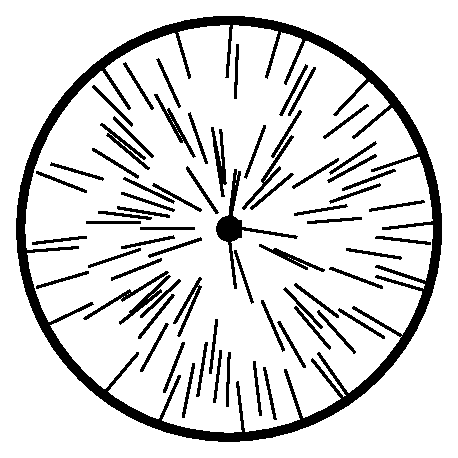
\includegraphics[height=.2\textwidth]{radial-cross}}
\subfigure{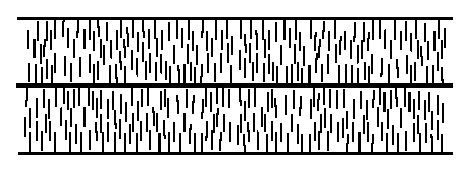
\includegraphics[height=.2\textwidth]{director-profile-radial}}
\caption{"Celni in stranski prerez nematskega vlakna z radialnim direktorskim profilom. }
\label{fig:fibre-radial-profile}
\end{figure}

Vrednosti parametrov, ki smo jih uporabili pri simulaciji, so na"steti v tabeli \ref{tab:parametri}. 

\begin{table}[!htb]
\centering
 \begin{tabular}{|c|c|}
  \hline
  Valovna dol"zina svetlobe & 480 nm \\
  Premer vlakna & 3 $\mu$m \\
  Enota diskretizacije & 40 nm \\
  \hline
  Redni lomni koli"cnik v vlaknu & 1,52 \\
  Izredni lomni koli"cnik v vlaknu & 1,68 \\
  Lomni koli"cni okoli"ske snovi & 1,33 \\
  \hline
  "Sirina grla laserskega sunka & 3 $\mu$m \\
  Trajanje sunka & 40 fs \\
  \hline
 \end{tabular}
 \vspace{2mm}
 \caption{Parametri materiala in laserskega sunka, uporabljeni pri izra"cunih}
 \label{tab:parametri}
\end{table}

Najprej smo v vlakno poslali kratek laserski sunek vidne svetlobe z valovno dol"zino 480 nm in trajanjem sunka 40 fs. 
Zaradi dvolomnosti teko"cega kristala smo opazili razcep sunka na dve komponenti oz. dva lastna na"cina "sirjenja svetlobe. 
Ker pa je direktorsko polje singularno, sta tudi polarizaciji obeh na"cinov singularni, kot prikazuje slika \ref{fig:pulse-p1-mode}. 

\begin{figure}[!htb]
 \centering
 \sunek{p1}
 \caption{Lastna na"cina "sirjenja svetlobe skozi vlakno z radialnim profilom direktorja ($s=+1$)}
 \label{fig:pulse-p1-mode}
\end{figure}

S slike takoj opazimo podobnost med polarizacijo svetlobe, zlasti pri po"casnej"sem nihajnem na"cinu (slika \ref{fig:pulse-p1-mode} desno), in direktorskim poljem. 
"Ce na polarizacijo $\vec P$ gledamo kot na enotski vektor z direktorsko simetrijo, lahko z ena"cbo (\ref{eq:winding-number}) obema na"cinoma priredimo ovojno "stevilo $+1$. 
Dodatno pa ima vsak izmed na"cinov po eno ravnino ravnino ni"celne intenzitete, kjer se polarizacija svetlobe obrne. 
V enem izmed na"cinov je ta ravnina navpi"cna, v drugem pa vodoravna. 
"Ce polarizacijo svetlobe na eni strani te ravnine obrnemo, dobimo pravi linijski defekt mo"ci $+1$. 

Direktorsko polje znotraj vlakna ima radialno simetrijo, saj se ne spremeni "ce vlakno vrtimo okrog svoje osi. 
To simetrijo pa zlomi vpadna svetloba, ki uvede preferen"cno smer, in sicer smer polarizacije. 
Po dolgem "casu v vlaknu mora svetlobni "zarek zadostiti obema simetrijama. 
Efektivno si oba na"cina na sliki \ref{fig:pulse-p1-mode} lahko predstavljamo kot defekta v polarizaciji z ovojnim "stevilom $+1$, ki jim odstranimo vse tiste dele, kjer bi polarizacija morala kazati pravokotno na vpadno polarizacijo. 

\section{Hiperboli"cni profil direktorja}

V vlaknu z radialnim direktorskim profilom opazimo tesno povezavo med simetrijo teko"cega kristala in polarizacijo svetlobe. 
Na podlagi tega lahko pri"cakujemo podobno povezavo tudi, "ce namesto defekta z ovojnim "stevilom $+1$ v sredino vlakna postavimo drug defekt. 
Z vektorskim poljem so kompatibilni le tak"sni s celo"stevilsko mo"cjo, zato smo najprej izbrali hiperboli"cni defekt z mo"cjo $s=-1$. 

Radialni direktoski profil znotraj vlakna opazimo eksperimentalno, ker sidranje na robu vlakna vsiljuje pravokotno smer direktorja. 
Druga"cnih direktorskih polj, na primer tak"snega s hiperboli"cnim defektom, pa ne moremo ustvariti samo z izbiro robnih pogojev. 
Poljuben direktorski profil je mogo"ce teko"cemu kristalu vsiliti z zunanjim poljem, nato pa ga stabilizirati s polimerizacijo \cite{dierking-polymer}. 

Kratek laserski sunek se podobno kot pri radialnem profilu razdeli na dva na"cina, ki sta skladna s simetrijo direktorja. 
Oba na"cina sta prikazana na sliki \ref{fig:pulse-m1-mode}. 

\begin{figure}[!htbp]
 \centering
  \sunek{m1}
 \caption{Lastna na"cina "sirjenja svetlobe skozi vlakno s hiperboli"cnim profilom direktorja ($s=-1$)}
 \label{fig:pulse-m1-mode}
\end{figure}

Obmo"cja z vi"sjo intenziteto svetlobe so razporejena enako kot na sliki \ref{fig:pulse-p1-mode}, polarizacijo svetlobe pa tvori defekt z ovojnim "stevilom $-1$. 
Spet sta vidni ravnini ni"celne intenzitete, kjer se smer polarizacije obrne. 

\section{Defekti s polovi"cno mo"cjo}

Radialni in hiperboli"cni profil direktorja znotraj teko"cekristalnega vlakna vsili svojo simetrijo polarizaciji svetlobe. 
Na mestih, kjer ta simetrija ni kompatibilna s polarizacijo vpadne svetlobe, pa se pojavijo obmo"cja ni"celne intenzitete svetlobe. 
V obeh primerih bi lahko z obratom polarizacije na delu vlakna dosegli, da polarizacija svetlobe tvori defekt s celo"stevilsko mo"cjo. 
Tak"sni defekti so kompatibilni z vektorskimi polji, kot je elektri"cno polje svetlobe. 
V teko"cem kristalu pa lahko ustvarimo tudi defekte s polcelo mo"cjo, ki jih prava vektorska polja ne morejo tvoriti. 
Ti so "se posebej zanimivi za eksperimentalno delo, saj se zaradi ni"zje energije pogosto pojavljajo v razli"cnih vzorcih teko"cih kristalov, ne samo v vlaknih. 

Simulirali smo "sirjenje svetlobe skozi teko"cekristalno vlakno, ki ima v osi linijski defekt z ovojnim "stevilom $s =\pm 1/2$. 
Izka"ze se, da se tudi v tem primeru laserski sunek razcepi na dva dela, ki ustrezata redni in izredni polarizaciji. 
V nasprotju z radialnim in hiperboli"cnim profilom pri propagaciji svetlobe skozi defekte s polovi"cno mo"cjo ne opazimo ravnin brez svetlobe. 
Znotraj vsakega lastnega na"cina je le eno intenzitetno obmo"cje. 
Simetrijski ravnini, opa"zeni pri celo"stevilskih defektih, nista kompatibilni s simetrijo defekta s polcelim ovojnim "stevilom. 
Spet pa so opazna temna obmo"cja, kjer bi morala biti polarizacija svetlobe pravokotna na vpadno polarizacijo. 

\begin{figure}[!htbp]
 \centering
  \begin{overpic}[width=.4\textwidth]{licp_p12_68}\put(2,90){\color{white} \large \bf (a)}\end{overpic} \hspace{1mm}
  \begin{overpic}[width=.4\textwidth]{licp_p12_78}\put(2,90){\color{white} \large \bf (b)}\end{overpic}
 \caption{Lastna na"cina "sirjenja svetlobe skozi vlakno z defektom z necelim ovojnim "stevilom $s=+1/2$}
 \label{fig:pulse-p12-mode}
\end{figure}

\begin{figure}[!htbp]
 \centering
  \begin{overpic}[width=.4\textwidth]{licp_m12_68}\put(2,90){\color{white} \large \bf (a)}\end{overpic} \hspace{1mm}
  \begin{overpic}[width=.4\textwidth]{licp_m12_78}\put(2,90){\color{white} \large \bf (b)}\end{overpic}
 \caption{Lastna na"cina "sirjenja svetlobe skozi vlakno z defektom z necelim ovojnim "stevilom $s=-1/2$}
 \label{fig:pulse-m12-mode}
\end{figure}


\section{Posplo"sitev in splo"sne zna"cilnosti}
Nekaj lastnosti lastnih na"cinov propagacije svetlobe lahko obrazlo"zimo s simetrijo. 
Polarizacija vpadne svetlobe je linearna in uniformna. 
Njeno ovojno "stevilo je enako 0, torej ima dvo"stevno rotacijsko os in dve zrcalni osi. 
"Ce je svetloba polarizirana v smeri osi $x$, sta zrcalni osi os $x$ in os $y$. 
Kak"sna izmed teh dve zrcalnih osi je prisotna tudi v direktorskem defektu, ne pa nujno obe. 
Polarizacija svetlobe znotraj vlakna bo obdr"zala vse simetrijske osi, ki so prisotne tako v vpadni svetlobe kot tudi v teko"cem kristalu. 

V zgorjih opa"zanjih lahko najdemo podobnosti; za propagacijo linearno polarizirane svetlobe vzdol"z nematskih defektnih linij velja:
\begin{itemize}
 \item Sunek linearno polarizirane svetlobe se vedno razdeli na dva lastna na"cina, ki ustrezata redni in izredni polarizaciji.
 \item Polarizacija svetlobe v obeh na"cinih tvori defekt z enakim ovojnim "stevilom kot defekt v teko"cem kristalu, "ce pri dolocitvi ovojnega stevila polarizacije predpostavimo simetrijo $\vec P \leftrightarrow -\vec P$ in gladek prehod "cez mesta z ni"celno intenziteto svetlobe. 
 \item V enem izmed na"cinov je polarizacija svetlobe vzporedna z direktorjem, v drugem pa je nanj pravokotna.
 \item V obmo"cjih, kjer bi po prej"snjem pravilu morala biti svetloba polarizirana pravokotna na vpadno polarizacijo, se pojavijo ``temna'' obmo"cja -- obmo"cja ni"celne intenzitete svetlobe.
 \item Lastna na"cina imata iste simetrijske ravnine, ki so presek simetrijskih ravnin teko"cega kristala in polarizacije vpadne svetlobe. 
\end{itemize}

S temi posplositvami lahko napovemo, kako se bo svetloba "sirila vzdolz nematskega vlakna s poljubnim linijskim defektom vzdol"z osi. 

\chapter{Stalna laserska svetloba}

Zelo kratki laserski sunki so zanimivi za teoreti"cno obravnavo, ker lahko z njimi najdemo lastne na"cine "sirjenja svetlobe po snovi. 
Z eksperimentalnega vidika pa so izjemno zahtevni, tako za ustvarjanje pulza kot za njegovo opazovanje. 
Sunek, uporabljen na zgornjih slikah je trajal le okrog 40 fs, kar je sicer v dosegu ultrahitrih femtosekundnih laserjev. 
Mnogo bolj enostavno pa je opazovanje z laserjem, ki sveti stalno s konstantno intenziteto. 

\section{Radialni profil direktorja}

Pri enakomernem laserskem "zarku je svetloba v vlaknu z radialnim profilom direktorja kombinacija obeh lastnih na"cinov, ki se "sirita z razli"cnima hitrostma. 
Frekvenca svetlobe je nespremenjena in zato enaka po celotnem vlaknu, opazimo pa mo"cno krajevno odvisnost oblike polja. 
Trenutne slike elektri"cnega polja znotraj vlakna so prikazane na sliki \ref{fig:p1-cont-snaps}. 

\begin{figure}[!ht]
\centering
\stalno{p1}{2}
 \caption{Posnetki elektri"cnega polja na razli"cnih mestih znotraj vlakna z radialnim direktorskim profilom ob stalni osvetlitvi. 
 Vidno je izmenjevanje konfiguracij z ovojnima "steviloma $s=0$ (a) in $s=+2$ (c). 
 Na sliki (b) je vmesno stanje, kjer je elektri"cno polje podobno kot pri defektu mo"ci $s=+1$.
 Direktorsko polje v vlaknu je prikazano na sliki (d).}
 \label{fig:p1-cont-snaps}
\end{figure}

\begin{comment}
\begin{figure}[!htbp]
 \subfigure{\includegraphics[height=130pt]{g_defect_0}}
 \subfigure{\includegraphics[height=130pt]{g_defect_2}}
 \subfigure{\includegraphics[height=130pt]{g_defect_4}}
 \caption{Shematski prikaz defektov z ovojnimi "stevili (od leve proti desni) $0$, $+1$ in $+2$. }
\end{figure}
\end{comment}

Na sliki je dobro vidno izmenjevanje konfiguracij elektri"cnega polja z ovojnima "steviloma $s=0$ in $s=+2$. 
Zaradi razlike v hitrosti propagacije se na nekaterih mestih v vlaknu oba valovna na"cina z ovojnim "stevilom $+1$ se"stejeta, na drugih pa od"stejeta. 
Rezultati nakazujejo, da se podobno zgodi tudi z defektom v polarizaciji svetlobe. 
Na prvem in zadnjem preseku na sliki \ref{fig:p1-cont-snaps} lahko vidimo defekt mo"ci $s=+2$, na drugi sliki z desne pa je vidna uniformna konfiguracija elektri"cnega polja brez defektov. 
Vmes, kot na primer na tretji sliki z desne, pa opazimo vmesno stanje. 
Konfiguracija ustreza defektu z ovojnim "stevilom $+1$, kjer zaradi nekompatibilnosti s smerjo polarizacija manjka del, kjer bi moralo biti polje v smeri $y$. 
Presek polja je zelo podoben lastnemu na"cinu vlakna, prikazanemu na desni strani slike \ref{fig:pulse-p1-mode}. 

\cleardoublepage
\section{Hiperboli"cni profil direktorja}

Podobno obna"sanje opazimo tudi v vlaknu s hiperboli"cnim direktorskim profilom, ki ima v osi defekt z ovojnim "stevilom $-1$. 
V tem primeru polarizacija svetlobe prehaja med na"cinoma z ovojnim "stevilom $0$ in $-2$, spet pa so opazna tudi vmesna stanja z ovojnim "stevilom $-1$. 
Primer svetlobnega polja v tak"snem vlaknu je na sliki \ref{fig:m1-cont-snaps}

\begin{figure}[!ht]
\centering
  \stalno{m1}{-2}
 \caption{Posnetki elektri"cnega polja na razli"cnih mestih znotraj vlakna s hiperboli"cnim direktorskim profilom ob stalni osvetlitvi. 
 Vidno je izmenjevanje konfiguracij z ovojnima "steviloma $s=0$ (a) in $s=-2$ (c). 
 Na sliki (b) je vmesno stanje, kjer je elektri"cno polje podobno kot pri defektu mo"ci $s=-1$.
 Direktorsko polje v vlaknu je prikazano na sliki (d).}
 \label{fig:m1-cont-snaps}
\end{figure}

\begin{comment}
\begin{figure}[!htbp]
 \subfigure{\includegraphics[height=130pt]{g_defect_0}}
 \subfigure{\includegraphics[height=130pt]{g_defect_-2}}
 \subfigure{\includegraphics[height=130pt]{g_defect_-4}}
 \caption{Shematski prikaz defektov z ovojnimi "stevili (od leve proti desni) $0$, $-1$ in $-2$. }
\end{figure}
\end{comment}

\section{Defekti s polovi"cno mo"cjo}

Nazadnje smo simulacijo ponovili tudi z vlaknom, v katerem ima ureditev teko"cega kristala defekt s polcelo mo"cjo. 
Tak"sen primer je "se posebej zanimiv, ker imata lastna na"cina le eno simetrijsko ravnino, in sicer tisto, ki vsebuje polarizacijo vpadne svetlobe. 

\begin{figure}[!ht]
\centering
  \stalno{p12}{1}
  \caption{Posnetki elektri"cnega polja na razli"cnih mestih znotraj vlakna z direktorskim profilom z defektom mo"ci $+1/2$ ob stalni osvetlitvi. 
  Vidno je izmenjevanje konfiguracij z ovojnimi "stevili $s=0$ (a), $s=+1/2$ (b) in $s=+1$ (c). 
  Z belo barvo so prikazane silnice elektri"cnega polja, njihova svetlost pa je sorazmerna z intenziteto svetlobe. 
  Rde"ce pu"s"cice prikazujejo trenutno elektri"cno polje. 
  Direktorsko polje v vlaknu je prikazano na sliki (d). }
 \label{fig:p12-cont-snaps}
\end{figure}

Na slikah lahko prepoznamo uniformno polje brez defektov (skrajno levi presek) in polje z defektom mo"ci $-1$ (drugi presek z leve). 
Za razlike od defekta mo"ci $1$, ki ga opazimo v vlaknu s hiperboli"cnim profilom, pa je na zgornji sliki jasno vidna tudi komponenta svetlobe s polarizacijo, ki je pravokotna na vpadno polarizacijo. 
"Cisto desen presek na sliki \ref{fig:m12-cont-snaps} prikazuje vmesno stanje z defektom mo"ci $-1/2$, kjer zopet manjka komponenta v smeri $y$. 

Podobno velja za defekt z ovojnim "stevilom $+1/2$, ki je prikazan na sliki \ref{fig:p12-cont-snaps}. 

\begin{figure}[!ht]
\centering
  \stalno{m12}{-1}
  \caption{Posnetki elektri"cnega polja na razli"cnih mestih znotraj vlakna z direktorskim profilom z defektom mo"ci $-1/2$ ob stalni osvetlitvi. 
  Vidno je izmenjevanje konfiguracij z ovojnimi "stevili $s=0$ (a), $s=-1/2$ (b) in $s=-1$ (c). 
  Z belo barvo so prikazane silnice elektri"cnega polja, njihova svetlost pa je sorazmerna z intenziteto svetlobe. 
  Rde"ce pu"s"cice prikazujejo trenutno elektri"cno polje. 
  Direktorsko polje v vlaknu je prikazano na sliki (d). }
 \label{fig:m12-cont-snaps}
\end{figure}

Na drugi sliki z leve je lepo viden radialen profil polarizacije svetlobe. 
Tako enakomerne radialne polarizacije ne moremo dobiti z radialnim profilom teko"cekristalnega direktorja. 
Z uporabo defekta s polovi"cno mo"cjo pa lahko "zarek linearno polarizirane laserske svetlobe pretvorimo v "zarek z radialno polarizacijo. 

Na podlagi rezultatov lahko zaklju"cimo, da polarizacija, pravokotna na vpadno, manjka le pri na"cinih oz. konfiguracijah polja, kjer polje tvori defekt z enako mo"cjo kot defekt v teko"cem kristalu. 
S konstantnim laserskim "zarkom dose"zemo se"stevanje obeh propagacijskih na"cinov, ki na dolo"cenih mestih v vlaknu privede do komponente s pravokotno polarizacijo. 
Tu je pomembno, da pri lastnih na"cinih ni vsa svetloba polarizirana vzporedno z vpadno polarizacijo.
Le tam, kjer bi zaradi topologije defekta morala biti polarizirana v pravokotni smeri, intenziteta svetlobe mo"cno pade. 
Pri konstantnem svetenju pa se lastni na"cini se"stejejo tako, da imajo ombo"cja, kjer topologija defekta narekuje polarizacijo v smeri, pravokotni na vpadno polarizacijo, enako intenziteto svetlobe kot okolica. 

\begin{comment}
\begin{figure}[!htbp]
 \subfigure{\includegraphics[height=130pt]{g_defect_0}}
 \subfigure{\includegraphics[height=130pt]{g_defect_-1}}
 \subfigure{\includegraphics[height=130pt]{g_defect_-2}}
 \caption{Shematski prikaz defektov z ovojnimi "stevili (od leve proti desni) $0$, $-1/2$ in $-1$. }
\end{figure}
\end{comment}

\section{Radialno polarizirana svetloba}
Radialno polarizirana svetloba je uporabna za laserske pasti \cite{radial-trap}.
Z radialno polariziranim "zarkom lahko ujamemo tudi delce, ki jih z linearno polarizirano svetlobo zelo te"zko, na primer mikroskopske kovinske delce.
Radialno polarizirano svetlobo je mo"zno fokusirati v piko velikosti $0,\!16\lambda^2$, kar je ob"cutno manj od meje $0,\!26\lambda^2$ za linearno polazirino svetlobo \cite{radial-focus, kozawa-sato-focal-spot}. 
S primerno dvolomnostjo teko"cega kristala in dol"zino vlakna lahko linijski defekt z ovojnim "stevilom $s=1/2$ slu"zi kot pretvornik med linearno in radialno polarizacijo svetlobe. 

"Ce "zelimo, da se lastna na"cina propagacije svetlobe po vlaknu z defektom mo"ci $1/2$ (na sliki \ref{fig:pulse-p12-mode}) se"stejeta v radialno polarizacijo, mora biti fazna razlika med njima pol nihaja. 
V vlaknu z dol"zino $d$ bo redni "zarek naredil $d/\lambda_o = d n_o/\lambda$ nihajev, izredni pa $d/\lambda_e = Ln_e/\lambda$ nihajev, kjer je $\lambda$ valovna dol"zina svetlobe v vakuumu. 
"Zeleno radialno polarizacijo bomo dobili, "ce bo razlika med "steviloma nihajev polcelo "stevilo. 
\begin{align}
  k + \frac{1}{2} &= \frac{d}{\lambda} \left( n_e - n_o \right) = \frac{d}{\lambda} \Delta n
\end{align}
kjer je $k$ poljubno celo "stevilo. Za tipi"cne vrednosti lomnih koli"cnikov v teko"cih kristalih in valovne dol"zine svetlobe lahko izra"cunamo optimalno dol"zino vlakna kot
\begin{align}
 d &= \frac{\lambda}{2\Delta n} \approx \frac{480~\mathrm{nm}}{2 \times 0,\!16} \approx 1,\!5~\mu\mathrm{m}
\end{align}
"ce izberemo vrednosti $k=1$. Ker je "stevilo $k$ poljubno, lahko isto stvar dose"zemo tudi z dalj"simi vlakni. 
Dol"zina, potrebna za pretvorbo iz linearne v radialno polarizacijo, se spremeni tudi ob uporabi teko"cega kristala z druga"cno dvolomnostjo ali laserja z drugo valovno dol"zino. 
Dvolomnost teko"cega kristala je odvisna od stopnje reda $S$ in s tem tudi od temperature, kar omogo"ca uravnavanje delovanja tak"sne naprave. 

\chapter{Zaklju"cek}

Implementirali smo numeri"cno metodo za modeliranje "sirjena svetlobe po opti"cno anizotropnih sredstvih, kot so teko"ci kristali. 
Metoda temelji na metodi kon"cnih diferenc v "casovni domeni (FDTD), ki svetlobo opi"se s "sestimi komponentami elektromagnetnih polj, njihov "casovni razvoj pa z Maxwellovimi ena"cbami. 
Izvori svetlobe so modelirani z robnim pogojem, na ostalih robovih pa je absorbirajo"ca plast, ki prepre"cuje odboj valovanja. 
Izbrali smo diskretizacijsko mre"zo, ki omogo"ca optimalno natan"cnost metode pri dolo"ceni ra"cunski zahtevnosti, hkrati pa omogo"ca modeliranje opti"cno anizotropnih snovi. 
Metodo smo uporabili na primerih, ki so dovolj zapleteni, da dajo netrivialne rezultate, hkrati pa so dovolj enostavni, da poznamo to"cne re"sitve. 
Pravilno napove odboj in lom valovanja ob prehodu v medij z druga"cnim lomnim koli"cnikom, prepustnost uniformne dvolomne plasti in prepovedani pas v enodimenzionalnem fotonskem kristalu. 
Kratek laserski sunek se v uniformnem nematskem vlaknu razdeli na dva dela, ki ustrezata redni in izredni polarizaciji svetlobe. 

Pri uporabi metode za modeliranje "sirjenja svetlobe po vlaknu z teko"cekristalno defektno linijo smo opazili zanimivo povezavo med topolo"skim defektom v teko"cem kristalu in topolo"skem defektu v polarizaciji svetlobe. 
Laserski sunek, ki ima na za"cetku linearno polarizacijo, razpade na dva lastna na"cina "sirjenja. 
Polarizacija svetlobe v vsakem izmed na"cinov tvori defekt, ki je po ovojnem "stevilu enak defektu v teko"cem kristalu. 
Na mestih, kjer simetrija defekta dolo"ca, da mora biti polarizacija svetlobe pravokotna na za"cetno polarizacijo, se pojavijo obmo"cja z ni"celno intenziteto. 
Tesna povezava med teko"cekristalnim direktorskim poljem in elektromagnetnim poljem velja tudi v primeru, ko je znotraj vlakna defekt s polovi"cno mo"cjo, ki ga polarizacija svetlobe kot pravi vektor ne more tvoriti. 

Opisana numeri"cna metoda je primerna za modeliranje opti"cno poljubno zapletenih snovi. 
Ker upo"steva vseh "sest komponent elektromagnetnih polj, pravilno deluje tudi v teko"cih kristalih z mo"cno krajevno odvisnostjo dvolomnosti, na primer v bli"zini defektov, kjer druge metode odpovejo. 
Ta metoda ponuja mnoge mo"znosti za nadaljnje raziskave, zlasti na podro"cju teko"cih kristalov. 
Med elektromagnetnim poljem in teko"cimi kristali velja dvosmerna sklopitev, ki jo bo mogo"ce upo"stevati s kombinacijo zgoraj opisane metode z obstoje"cimi programi za izra"cun ureditve teko"cih kristalov v prisotnosti zunanjih polj. 
Vsaj nekatere rezultate numeri"cne metode bo mo"zno eksperimentalno preveriti, npr. s tvorbo teko"cekristalnih vlaken z radialnim direktorskim profilom. 
Zanimiv rezultat je tudi napoved novega na"cina za pretvarjanje polarizacije svetlobe iz linearne v radialno, ki predstavlja nov izziv za eksperimentalno delo. 

\bibliographystyle{zumer}
\bibliography{magisterij}

\end{document}
